%\documentclass[final,1p,times]{elsarticle}
%\documentclass[twocolumn]{elsarticle}
\documentclass[a4paper,10pt,twocolumn,preprint,3p]{elsarticle}

\usepackage{graphics}
\usepackage{amssymb}
\usepackage{amsmath}
\usepackage[dvips]{epsfig}
\usepackage[latin1]{inputenc}
\usepackage{url}
\usepackage{appendix}

%\def\CC{{C\hspace{-.05em}\raisebox{.4ex}{\tiny\bf ++}}~}
%\addtolength{\textfloatsep}{-0.5cm}
%\addtolength{\intextsep}{-0.5cm}


\journal{Knowledge-Based Systems}

\begin{document}

\begin{frontmatter}

%%%%%%%%%%%%%%%% Titulo %%%%%%%%%%%%%%%
\title{Applying Computational Intelligence Methods for Predicting the Sales of Newly Published Books in a Real Editorial Business Management Environment} 


%\setlength\textwidth\columnwidth


%%%%%%%%%%%%%%%% autores %%%%%%%%%%%%%%
\author[ugr]{Pedro A. Castillo}
\ead{pacv@ugr.es}
\author[ugr]{Antonio M. Mora}
\ead{amorag@geneura.ugr.es}
\author[abd]{Hossam Faris}
\ead{hossam.faris@ju.edu.jo}
\author[ugr]{J.J. Merelo}
\ead{jmerelo@geneura.ugr.es}
\author[ugr]{Pablo Garc\'{\i}a-S\'anchez}
\ead{pablogarcia@ugr.es}
\author[ugr]{Antonio J. Fern\'andez-Ares}
\ead{antares.es@gmail.com}
\author[ugr]{Paloma De las Cuevas}
\ead{palomacd@ugr.es}
\author[ugr]{Mar\'ia I. Garc\'ia-Arenas}
\ead{mgarenas@ugr.es}


\address[ugr]{Department of Computer Architecture and Computer Technology, ETSIIT and CITIC \\
University of Granada, Granada, Spain. Tel: +34958241778. Fax: +34958248993}
\address[abd]{Business Information Technology Department, King Abdullah II School for Information Technology \\
The University of Jordan, Amman, Jordan}

%%%%%%%%%%%%%%%%%%%%%%%%%%%%%%%%%%%%%%%%%%%%%%%%%%%%%%%%%%%%%%
\begin{abstract}
When a new book is launched the publisher faces the problem of how
many books should be printed for delivery to bookstores; printing too 
many is the main issue, since it implies a loss of investment due to
inventory excess, but printing too few will also have a negative economic impact. 
In this paper, we are tackling the problem of predicting total sales 
in order to print the right amount of books and doing so even before the book 
has reached the stores. A real dataset including the complete sales data for 
books published in Spain across several years has been used.
We have conducted an analysis in three stages: an initial exploratory analysis, 
by means of data visualisation techniques; a feature selection process, using 
different techniques to find out what are the variables that have more impact on sales; 
and a regression or prediction stage, in which a set of machine learning methods 
has been applied to create forecasting models for book sales. 
The obtained models are able to predict sales from pre-publication data with
remarkable accuracy, and can be visualised as simple decision trees. 
Thus, these can be used as decision-aid tools for publishers, which can provide 
a reliable guidance on the decision process of publishing a book. 
This is also shown in the paper by addressing four example cases of representative 
publishers, regarding their number of sales and the number of different books they sell.
\end{abstract}

\begin{keyword}
%% keywords here, in the form: keyword \sep keyword
Book sales forecasting \sep Decision-aid models \sep Feature selection \sep Regression  
%% MSC codes here, in the form: \MSC code \sep code
%% or \MSC[2008] code \sep code (2000 is the default)
\end{keyword}

\end{frontmatter}


%********************************************************************************

\section{Introduction}

Publishing a book, in the same way as releasing any other cultural product with a physical substrate, implies several types of risks and costs due to
the complexity, and derived expenses, of its processes of production,
distribution, and storage. Most of these costs are associated
with the number of books actually printed, the so called {\em print run}. But the problem is further complicated for completely new products, in the sense that they have been written by an unknown author or deal with a new topic with no track record. In order to make the print run as close as possible to actual sales, it is essential to have an estimation of those sales; that is the challenge we are taking in this paper. 

In general, forecasting the sales of cultural products can
only be based on the knowledge obtained from sales of other, similar, ones,
but the definition of ``similar'' itself is fuzzy and, sometimes,
subjective. Even if the author or the topic is known, making accurate
estimations of future sales of the new product is quite difficult, and
extremely important, so that production runs follow predicted sales. 
Indeed, several studies have demonstrated that improving sales
predictions, that is reducing the error in estimated sales, results in an enhancement in the whole production process \cite{Fildes2010,Saeed2008}, so not only the costs associated with the book itself are affected.

Within the general area of cultural products, the problem of
predicting sales is specially acute for book publishers who, among other
providers of content in physical form, release new {\em products} more frequently than
other industries, so that they face the problem of predicting sales quite often. The issue, in this case, is to print an adequate number of copies but not too many, as the unsold volumes will lead to losses and sunk inventory cost, 
whereas if the number of printed copies was not enough, a new print
run can always be made, but this will result in temporary losses due to a lack of supply or in bad marketing for the customers, for instance. However, in practice predicting lower sales than the actual ones is not such a big problem because the new print run is ordered before the inventory is exhausted; nevertheless, this new print run presents the same problem as the
initial one of printing only as many as forecasted, although its cost
is not as high as the initial one.

Despite the fact that errors in one or the other direction do not have
the same impact, it is extremely important to develop an accurate
predictive method 
which could forecast the future sales a new book will achieve, in
order to optimise production schedules, improve the publishing company
profits and minimise losses \cite{Zhao2001}. This is the main objective of this paper.

In Spain, the process of releasing a book goes like this: the
publisher decides, based on past experience, how many books to
print. These books are distributed to points of sale, but also given
out to reviewers and literary magazines; the number of these will
depend on how many were printed. Sometimes books go to
the {\em novelty} table of the bookstore, that is, they are prominently displayed, shown in the window, or highlighted using props or other 
%Pablo: rephrasing and removing comas
kind of advertisement. From these displays they then move to shelves
or, in some cases and eventually, to storage. Books stay for sale in the store as long as the publisher or the store wants or until the bookseller decides to return them to the publisher. Books returned to the publisher are pulped, sold back or given to the author, or finally distributed in used-books channels such as book stalls or second-hand bookstores. If the print run has been fully
distributed and there are more requests from bookstores, on the other
hand, a new print run is made and distributed to these shops. 
Even if the process has changed slightly 
in the last few years since Amazon started to sell in Spain, in the
sense that many books are sold through this new channel and do not
undergo the cycle novelty table-shelf-storage-back to publisher, which
actually happened {\em after} the data used for this paper was
collected, it roughly stays the same. Other countries will have a
similar model, although the scale will be different. 

Our intention in this paper is to find out the main factors influencing
sales in order to create a \textit{tool} that the publisher can use to decide how many books should be printed, as well as how to leverage these printed
copies to maximize sales using the decision variables under his
control. That is why, using data obtained from a company that sells
software for publishers, we analyse them and compute predictive models that can be mainly used as decision-aid tools for book publishers. With these models, publishers will be able to combine their expert knowledge about the market with the created forecasting models in order to get a reliable estimation of book
sales, and, based on it, act consequently in order to maximize the books sold for a particular print run. 

This will improve the current decision flow that the publishers follow, which consist in analysing (in a subjective way) the quality of the book and its features (author, genre, etc), and take a `fuzzy' decision roughly between printing 300 copies (standard book) or 5000 (best seller).

This process might be tedious, especially when the amount of data is quite large. Moreover, different experts can reach different predictions from the same dataset \cite{Sanders1994}. 

With these issues in mind, in this paper, we firstly present an analysis on a real dataset, provided by the Spanish publishing company Trevenque Editorial S.L.\footnote{{\tt http://editorial.trevenque.es}\\ Trevenque offers management systems and services for bookshops, publishers, and distributors}.
This study has been conducted by means of data mining and visualisation techniques. Then, a feature selection process is performed using three different methods, in order to find out what are the relevant variables describing a book in the prediction, or estimation, procedure. 
% (Paloma) Why brackets? Suggestions:
% relevant variables describing a book in the prediction or regression procedure
% relevant variables describing a book in the prediction, or regression, procedure
% relevant variables describing a book in the prediction (regression) procedure <- here brackets are ok (me thinks)
% Antonio - I have chosen a better option for not repeating 'regression' in the following sentence
This procedure is performed by applying a set of regression algorithms to the different datasets (those with a different number of variables), yielding a set of models which could be used as the desired tool. 

Given this, the main contribution of this paper to the state of the art is the development of the aforementioned methodology to process book sales data, in which: firstly, the most relevant variables are identified, and then, these variables are considered to `refine' the data in order to conduct accurate predictions on future sales. To our knowledge this is the first work in which regression methods have been applied to estimate sales for new launched books. Moreover, as stated before, we have used in the study a real dataset of book sales (related to the Spanish market), which is another point to remark.

The value of this methodology is contrasted considering four different
publishing companies being representative as top sellers, mid-range
sellers, the most varied, and one which sells a medium amount of
different books. From this, we draw insight on what are the important
factors when selling a book and some rule of thumbs extracted from the
prediction methods.


% (Paloma) From here:
%Usually, the company's expert sales managers analysed historical data
%and applied their knowledge on external variables to compute correct
%estimations (predictions); for instance, they can decide increasing or
%decreasing the sales forecast based on season or sales period. 
%Nevertheless, just carrying out the analysis and forecasting process
%as a human expert may lead to imprecise predictions, and they may not
%take all the variables into account.
% (Paloma) to here, is repeating all over again the process of deciding how many books to print. I think this paragraph should be unified somehow with the previous explanations and to re-order, because the previous paragraph seems like the end of the introduction, but then we go deep in the explanations again... It's not an easy read :(
% Antonio - removed and fused/reordered


The rest of this paper is structured as follows: next, Section \ref{sec:soa} presents a comprehensive review of the approaches found in the bibliography related to sales prediction in similar scopes, and shows a set of definitions of the regression methods applied in the paper as well as the evaluation metrics considered.
Then, Section \ref{sec:problem} introduces the problem of the estimation of print run
% (Paloma) Guys, 'print run' is written a total of 28 times:
% 23 are in the 'print-run' form
% 5 are 'print-run' (with a dash), of which one is inside the list of variables. But what about the rest inside text? Shouldn't they go ALL either with or without the dash?
% Antonio - I have replaced all of them by 'print run' as it seems to be the correct one
for new books, along with a description of the considered dataset.
Section \ref{sec:methodology} details the methodology considered in the study. These are reported in Section \ref{sec:experiments}, which is also devoted to analyse the obtained results in feature selection and book sales forecasting using different datasets, with different amounts of features, for all the publishing companies. Obtained results for the four considered special cases are commented in Section \ref{sec:example_cases}. Finally, conclusions and future lines of work are presented in Section \ref{sec:conclusionsAndFutureWork}. 


%********************************************************************************
\section{Background and State of the art on sales forecasting} 
\label{sec:soa}

As far as we know, no previous attempt can be found in the literature in which prediction methods have been applied to estimate sales for new launched books in a whole country market. However, similar techniques to those proposed in this paper, e.g. regression models \cite{Papalexopoulos1990}, neural networks \cite{Yoo1999} or fuzzy systems \cite{Mastorocostas2001}, have been applied to solve sales prediction problems in other industrial sectors.

Specifically, time-series prediction methods
\cite{Chu2003,Brown1959,Winters1960,Box1969,Papalexopoulos1990,KayacanUK10} 
is perhaps the most used technique to tackle sales forecasting
problems, although the efficiency of these techniques strongly depends on the 
field of application and the correctness of the problem data. However, since 
they require a large amount of data for predicting sales, these methods are not 
the most suitable for this task \cite{ChingChin2010}. 
Moreover, this kind of methods cannot be applied before the book is published, 
as is the objective of this paper. 
In this case, just a few variables are known in advance (pre-sales data)
\cite{ChingChin2010,FaderHardie2005,Madsen2008}, and some of 
them are categorical, which makes them harder to process, even more if 
the number of categories is high. As stated in those works, given these issues, 
finding adequate forecasting techniques and selecting the best method to use 
is also a problem.
An additional issue makes this a complex problem, since the predictions are 
influenced by external variables that must be taken into account, such as
seasonality, promotions, or fashions that expert managers might
subjectively apply \cite{Lapide1999,ChernWSF15}.
% [pedro] I have not found a reference. This is based on what Santiago told us.
% We can remove next sentence if you think it only should appear together with a reference.
For this reason, usually the methods used to predict book sales have
been generally based on experts' experience, who analyse data about sales and, 
taking into account their knowledge of the industry, their experience, 
and their perception about trends, could make decisions on the companies 
production, i.e. how many books should be printed when a new book is published. 

Recently, some works have proposed analysing relationships between on-line 
information and book sales \cite{Moon2010ICSSSM,Moon2010ICEC}. 
Specifically, Moon et al. propose using the number of blog references as an 
indicator of the success of a book, and thus, its sales. 
Obtained results confirm relationships between the number of blog references 
and book sales, and at the same time different sales patterns are observed 
by analysing books in series (the first book published takes the longest period 
to achieve every single sales scale, while the second book takes the second 
longest period, and so on).

In general, historical data are used to make time series, as well as for extracting common patterns and obtaining accurate predictions from them.
However, in the case of new products, such as the issue of new books, past patterns are difficult to observe as there is no available historical sales data 
\cite{ChingChin2010}. Thus, only pre-sales data are available in this problem, i.e. variables known before the book is on sale.

In order to deal with this issue, i.e. forecasting sales of new products, some authors have used different data mining methods, such as 
``Accurate Response'', an approach for demand estimation and production planning \cite{Hammond1990}, 
data clustering and fuzzy neural networks \cite{Chang2009} or 
extreme learning machine with adaptive metrics of inputs \cite{Xia2012}. 
%
In the same line, Thomassey et al. \cite{SThomassey2014} proposed using a 
clustering method together with decision trees for sales forecasting in 
textile-apparel fashion industry, a very similar issue to the new book 
publishing problem.
The same problem was previously faced by Xia et al. \cite{Xia2012} using a 
forecasting method based on extreme machine learning with adaptive metrics of inputs.

The complexity of this problem relies on the lack of historical data, on the 
short lifetime of the majority of items, and on the influence of variables such 
as promotions, fashions, or economic environment
 \cite{Thomassey2012,Xia2012,SThomassey2014}, as mentioned above.

Ching et al. propose in \cite{ChingChin2010} a decision-support system for new 
product sales forecasting to solve three real-world sales forecasting 
problems, namely: new tea, cosmetics, and soft drink products. 
In that study, products are classified based on their sales patterns, so it is 
assumed that products in the same class would follow a similar sales pattern. 
However, as the authors state, the proposed system can not deal with qualitative 
data related to the products. Moreover, real-world cases, such as consumer 
electronics and fashion products, should be deeply analysed, as these industries 
present/launch new products every season. 

On the other hand, in those cases where historical data are available, classical time series forecasting methods have been applied, such as in \cite{Chang2009}, 
where a hybrid model integrating K-Means and fuzzy neural networks to forecast 
the future sales of a printed circuit board is proposed.
A similar method is described by Chern et al. \cite{ChernWSF15}, who analysed 
historical data throughout online reviews, reviewer characteristics, and review 
influences to understand how electronic `word-of-mouth' influences product sales. 
In this case, the proposed method is suitable for those sales forecasting problems with a big amount of online reviews and historical data.

Thus, taking into account the kind of problem we address in this
paper, i.e. the prediction of sales of a new product for which no
historical data are available, the classical forecasting methods based
on time-series are not adequate, although they can obviously be used once 
the book has been launched for sale. 
In our work the relevant variables in the prediction of sales are identified
by means of data visualisation and feature selection methods. 
Then, machine learning techniques are applied to predict sales and to infer 
the ideal print run of a book.
In addition, since publishers need models to explain obtained predictions, 
`black box' forecasting methods may not be suitable, so models based
on decision rules have been tested as an alternative. 


%********************************************************************************
\section{Problem description}
\label{sec:problem}

The problem to solve in this work is the forecasting of sales for new
launched books in the Spanish market, considering a set of `pre-sales
variables' or at least variables that are under the control of the
publisher before the book is going to be released to bookstores. The
objective is to offer a tool for publishers which will help them to
decide the best print run for a new book before its publication
process starts. This is a forecasting problem for which no specific
historical data are available and thus it is not simply a matter of
analyzing a time series, instead, we have considered data about other,
previously published, books and have taken as reference a set of
variables (or features), 
related to the book publication process. 

\begin{table*}[!ht]
\caption{Parameters describing a book, provided by the company Trevenque S.L.}
\label{tabla:paramsOrig50}
\begin{center}
\begin{tabular}{|c|c|}
\hline 

\begin{minipage}{2.45in}\begin{small}
 \begin{verbatim}
reference
author
retail price
subject1
subject2
subject3
publisher
collection
bookbinding
print run
total sales
dept stores sales
sales through delegates
rest of sales
total sales 1st year
mall sales 1st year
delegates sales 1st year
rest of sales 1st year
total distributed
distributed through dept stores
distributed through delegates
distributed - rest
total distributed 1st year
distrib. through dept stores 1st year
distrib. through delegates 1st year
\end{verbatim}
\end{small} \end{minipage}     & 

\begin{minipage}{2.3in} \begin{small}
\begin{verbatim}
rest of distributed 1st year
reprints
number of reprints
total returns
returns - dept stores
delegates returns
rest of returns
total returns 1st year
returns - dept stores 1st year
delegates returns 1st year
rest of returns 1st year
gifts
units distributed as novelty
total points of sale
points of sale - dept stores
delegates points of sale
rest of points of sale
total points of sale 1st year
dept stores points of sale 1st year
delegates points of sale 1st year
rest of points of sale 1st year
weeks for sale
positive sales environment
medium sales environment
negative sales environment
\end{verbatim}
\end{small} \end{minipage}    \\

\hline
\end{tabular}
\end{center}
\end{table*}


The training dataset includes historical data about 6083 books
published in Spain for several years, with an initial set of 50
variables per pattern. It has been provided by the Spanish publishing
company Trevenque Editorial S.L. Table \ref{tabla:paramsOrig50} shows the initial set of variables describing each book. 

Starting from these raw data, a preprocessing method has been performed in order to remove incorrect or incoherent patterns, such as those with null values in required variables, or with negative sales, for instance. 
Furthermore, the initial set of variables, presented in Table \ref{tabla:paramsOrig50}, has been reduced by an expert to use just those that can be known before a new book is launched, i.e. \textit{pre-sales data}. 
%Thus, their value do not depend on the book sales. 
The selected subset of features is described in Table \ref{tabla:params_pre_sales}.


\begin{table*}
\caption{Considered pre-sales features and their types. The third column shows
 the names of the variables used in the applied methods, and the last one indicates if they have been used as an input (independent) or an output (dependent) variable.} 
\label{tabla:params_pre_sales}
\begin{center}
\resizebox{14cm}{!}{
\begin{tabular}{|c|l|l|c|c|}
\hline 
No. & Feature Name & Variable & Type & In/Out\\
\hline 
1 & retail price (when launched) & \texttt{ret\_price} & numerical & input\\
2 & main subject (code) & \texttt{subject1} & numerical & input\\
3 & publisher + collection (joint code) & \texttt{collection} & categorical & input\\
4 & bookbinding (code) & \texttt{binding} & categorical & input\\
5 & gifts (promotional books) & \texttt{gifts} & numerical & input\\
6 & units distributed as novelty & \texttt{distrib\_novelty} & numerical & input\\
7 & total number of points of sale & \texttt{tot\_points\_sale} & numerical & input\\
8 & total number of points of sale (1st year) & \texttt{tot\_points\_sale\_1st\_year} & numerical & input\\
9 & weeks on sale & \texttt{weeks\_sale} & numerical & input\\
10 & print run & \texttt{print\_run} & numerical & input\\
\hline 
\hline
11 & total sales & \texttt{total\_sales} & numerical & output\\
\hline 
\end{tabular}
}
\end{center}
\end{table*}

As it can be seen in this table, \texttt{total\_sales} is the output
variable, so it is the objective of the prediction methods. {\tt
 total\_sales} is a variable percentage of the {\tt print\_run}, and
thus there is obviously some correlation between them, which might
prevent us from using it to predict sales; it is quite obvious that
just increasing the print run, by itself, will not boost
sales. However, several of the other variables include implicitly a
certain size of the print run; for instance, you have to actually
print books to distribute them as novelty and at least one, for every
point of sale, so including the print run makes sense to get more
accurate estimates of the total sales that you are going to obtain out
of the total print run and check its influence on the overall sales
volume. Once this is included in the model and also as part of the
tree nodes, changing the print run might give the publisher an idea of
how many books are going to be actually sold out of that print run,
and taking that into account decide on the actual number of books that
are going to be printed. Just to be clear, printing books does not
%PABLO: that "Just to be clear" is too informal
actually sell them, but it is obviously necessary to print books
before you sell them, and once you have to do it, the publisher might
make decisions on printing a few more and check, with this model, what
would be the influence in sales if, for instance, you decide to send
more books to every point of sale or distribute more in novelty. We 
%PABLO: previous phrase is toooooo large, please divide
will come back to this choice later on when examining the resulting
models. 

Initially, there were three different features describing the subjects
and subsubjects of every book \texttt{subject1,2,3} (see Table
\ref{tabla:paramsOrig50}), but for most of the patterns (books) there
is no value for \texttt{subjects2} and \texttt{3}, so we have discarded 
these features.   

With regard to the feature \texttt{publisher}, it has been removed from the 
final dataset since it is indeed included in the code of \texttt{collection}. 
In addition, we think it is not really relevant to the accuracy of the models 
and, moreover, publishers probably will not want to use the results of other 
publishing companies for predicting their own sales.

Therefore, in order to create simpler and more accurate prediction
models, and with the aim to provide them as a useful decision-aid tool
for the publisher, we have transformed the categorical variable
\texttt{subject1} into a numerical one, considering it refers to a
code of the Dewey Decimal Classification system for books
\cite{wiki:dewey}, and the existing similarity relationship between
the books inside a class or subclass. So, for instance, all the books
inside subdivisions of class 200, `Religion', are considered as
similar regarding their topics, so they could be also close in terms
of distance. The same reasoning can be applied to subclasses. 

In this prediction problem there are other external variables that also affect 
the sales of a new book \cite{Little1998}, such as those related to seasonality, trends, or promotions, that classical prediction methods can not deal with, since they are not included in the dataset due to the difficulty to model them. 
However, an expert can consider them to modify the forecast obtained by 
the automatic method \cite{Armstrong2001}. Even publishing companies tend to define rules or  indexes to subjectively adjust the results of prediction based on external data. 
Thus, the proposed method will analyse the provided data and
variables and will yield a forecast of sales according to them. This
result could be used as a reference for a human expert, who would
consider it for his or her own prediction process. 


%********************************************************************************
\section{Methodology}
\label{sec:methodology}

There is not a standard methodology to solve the general problem of sales forecasting. However, the steps we have followed in this paper are those usually applied in a Knowledge Discovery in Databases (KDD) process \cite{fayyad1996data}. Figure \ref{fig:methodology} summarizes these steps.

\begin{figure}[!ht] 
\begin{center}
  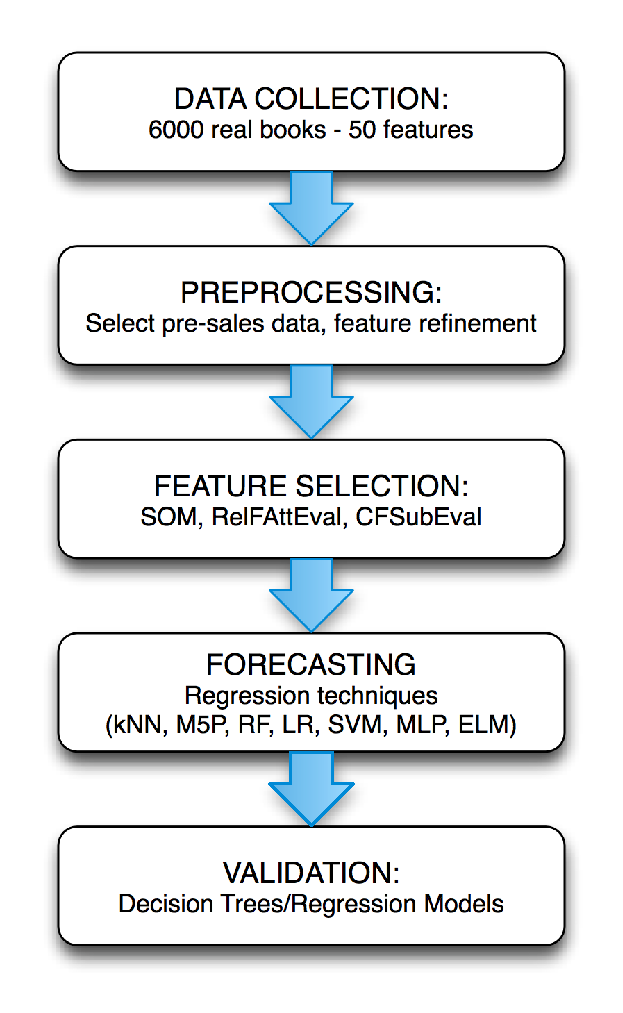
\epsfig{file=metodologia.eps,width=5.5cm}
\caption{Steps followed in the proposed methodology.}
\label{fig:methodology}
\end{center}
\end{figure}


Therefore, after the data has been \textit{collected} and initially \textit{preprocessed} (as described in the previous section), other preprocessing techniques have been applied, such as \textit{Feature Selection} (FS) \cite{kittler1986feature}, since it is an effective dimensionality reduction technique, able to discard less relevant or non-useful features \cite{Krishnapuram2004,Chen2011_FS_PTS}.

FS methods check the relevance of all the variables of the patterns, aiming to reduce the set of features on a dataset, in order to obtain intelligible models, in a lesser amount of time due to their lower complexity, and usually without accuracy loss.
This task may also help to identify leading indicators to be considered 
by a human expert to make predictions.
At this stage of the methodology, both numerical and visualisation-based approaches have been applied, in order to select the best set of variables for the forecasting methods. These are described in Section \ref{subsec:fs_techniques}. 

After this process has been conducted, different rule-based, tree-based and numerical \textit{forecasting methods} have been applied on the dataset. They are regression techniques and have been described in Section \ref{subsec:regression_methods}.

As a result of the previous step, several prediction models are obtained for the whole dataset. These have been \textit{evaluated} by means of the metrics described in Section \ref{subsec:evaluation_metrics}, and also \textit{analysed} in the experiments (Section \ref{sec:experiments}).

After this, the same methodology has been applied to some specific cases of publishing companies in order to \textit{validate} the proposal (Section \ref{sec:example_cases}). To this end, also specific interpretable models have been created as a final result of the work (Section \ref{subsec:decision_trees}). 

In the following sections, the main techniques to be applied on these steps are described, along with the evaluation metrics computed to value the generated prediction models.

%-------------------------------------------------
\subsection{Feature selection techniques}
\label{subsec:fs_techniques}

The aim of these algorithms is exploring the space of attributes to find out 
which subset of them yields the best results in a regression or prediction 
problem. To this end, the features describing every pattern are analysed. 
In this case, among the variables describing a new book, some may affect 
predictions as they provide information, while others may not be necessary 
and even redundant.

The application of FS also aims to reduce the complexity of the obtained 
forecasting models themselves, which, in turn, implies a reduction in the 
computational time for building these models. This has been a key 
factor in this work, because one of the objectives is to obtain `easily' 
interpretable decision models, which can be useful for human experts (publishers).
Regarding the algorithm, running time grows with the number of
features, making it impractical for problems with a large number of features 
\cite{Selvakuberan2008}; however, this is a secondary objective of this work.

FS is one of the ways of performing a feature reduction, the other one is 
feature extraction \cite{kittler1986feature}. 
Feature extraction is a `transformation-based approach', therefore
it transforms the original meaning of the features. This method
involves creating a subset of new features by combining the
existing ones; thus it is employed when the semantics of the
original dataset will not be needed by any future process. On the
contrary, FS attempts to retain the meaning of the
original feature set. It is part of what is called semantic-preserving
techniques, known as `selection-based approaches' \cite{liu1998feature}. 
In the problem this work addresses, it is very important to maintain the 
semantics of the initial variables set, and therefore just FS methods 
have been applied. 

We have used some numerical FS methods included in Weka software \cite{Hall2009,Witten2011}. This tool separates the process into two parts:

\begin{itemize}
  \item Attribute evaluator: This is the method by which the feature subsets are assessed. In this work, both a correlation-based feature subset evaluation method ({\tt CfsSubsetEval}) and an adaptation of relief for attribute estimation ({\tt ReliefFAttributeEval}) evaluation method are used. 
  
  The Correlation Feature Selection (CFS) method evaluates subsets of features/variables on the basis of the hypothesis made by Hall in \cite{Hall1998}, ``A good feature subset is one that  contains features highly correlated with
(predictive of) the class, yet uncorrelated with (not predictive of) each other''. This evaluator needs the numeric features to be transformed to nominal features first, by being discretized.
The CFS evaluation function measures the ``merit'' of the subsets, which depend on the mean feature-class correlation, and the average feature-feature intercorrelation. For continuous class problems (regression), the correlation between the attributes is estimated based on a standard linear correlation
using the Pearson's correlation coefficient as given in Equation \ref{eq:corr} \cite{hall2000correlation}. 

\begin{equation}
r_{XY}=\frac{\sum xy}{n\sigma_{x}\sigma_{y}}
\label{eq:corr}
\end{equation}


Where $X$ and $Y$ are two continuous variables expressed in terms
of deviation. 

``ReliefF'' is the second evaluator used in this work. It is important to note 
we have applied the Weka's implementation of the ReliefF algorithm for regression problems. This relief method is an updated version, called Regressional ReliefF or RReliefF for short \cite{RobnikSikonja1997}, of the original ReliefF by Kira \& Rendell \cite{Kira1992}. The algorithm works by evaluating single attributes, and not whole subsets of attributes as CFS does. Also, it is applicable even working with both nominal and numeric features, without the need for transformations. For this algorithm, the weight of an attribute depends on the difference of an attribute value inside an instance with its neighbours, being these the nearest instance of the same class, and the nearest of the different class. Therefore, a good attribute is that which gives similar values for instances of the same class, and different values for instances of different class.
 \item Search method: This describes the structured way in which the set of possible feature subsets is studied, based on the results of the evaluator. With regard to the used search criteria, it is important to take into account that CFS evaluates attribute subsets, and Relief evaluates attributes separately.

For this reason, the search method used with CFS has been BestFirst, that searches the space of feature subsets by greedy hill-climbing augmented with a backtracking facility. On the other hand, Ranker is the searching criteria used with the Relief evaluator. This method ranks features by their individual evaluations.
\end{itemize}

In addition, in order to reduce the dimensionality of the input data
and to choose an appropriate set of variables, the Self-Organizing Map
(SOM) \cite{kohonen1998} method has also been applied as a `subjective' 
(based on expert's opinion) FS technique based on the visualisation of the 
data as a set of 2D planes (one per feature of the dataset), and their 
interpretation for finding out relationships between these features.

SOM is a type of unsupervised neural network inspired by the
topographical organisation of the sensory cortex of human brain
\cite{kohonen1998}. It maps highly dimensional data into a lower
dimensional space where similar data patterns are located in more
adjacent areas on the grid. 

This method is normally used as a data visualization tool, since it allows 
to project any multi-variated dataset in a two-dimensional display, 
so an expert can detect topological relations among its neurons and thus 
make inferences or find interesting relationships on the input dataset 
(such as clusters, for instance).

Basically, SOM consists of two layers: input and output layer, also
known as Kohonen, layer. Input layer is fully connected with the 
Kohen layer which is usually a two dimensional grid of neurons
(i.e. units). This means that every neuron is linked to every input in
the input layer. 

SOM follows an iterative process applied in two stages: First, the
weights of the network are initialised randomly, then the n-dimensional
input vectors are presented to the network sequentially so the
distance between the weights of the neurons and the inputs are
computed using the simple Euclidean distance; in the second stage, the
neuron which has the shortest distance with the presented input vector
is updated along with the neurons in its neighbourhood. 
This neuron is called the best matching unit (BMU). 
The goal of the learning process is to minimise the neighbourhood distance 
in the output clusters.  

Once the SOM learning process is finished, a visual representation technique, 
named the Unified distance matrix (U-matrix) \cite{UmatUlts}, has been applied. 
This method uses the obtained codevectors (vectors of variables of the problem) 
as data source, and generates a matrix where each component is a distance 
measure between two adjacent neurons. In the U-matrix, the distance between 
adjacent neurons is measured and assigned different colours. Different colours 
between neurons indicate large distances (boundaries) while similar colours 
represent close areas (clusters).

%---

This method is usually applied to analyse data as similar items tend to be 
mapped close together, while those items dissimilar, are mapped apart.
Also, the SOM graph represents and highlight very clearly those
regions, or clusters, with high training sample concentration and fewer
where the samples are scarce. U-Matrix graph, together with the projection 
of variables into separate planes, the so-called component planes analysis 
(that SOM yields), will aid an expert to identify the most relevant features 
on every cluster, i.e. those with a higher influence on the creation of that 
cluster.

These FS techniques have been applied in Section \ref{subsec:feature_selection}, including a comparison between all of them.


%-------------------------------------------------
\subsection{Regression methods}
\label{subsec:regression_methods}

As previously stated, there are many prediction algorithms available in the 
literature, each one with a different parameter set that may affect the 
obtained results.

However, as in the case of new books only some descriptive data are available,
compared to those cases in which historical data on sales of published books 
is available, not all forecasting methods can be used in this specific problem.

Thus, in this research six forecasting methods, based on the State of the Art 
literature review (see above, Section \ref{sec:soa}) 
\cite{Madsen2008,ChingChin2010,Thomassey2012,Xia2012,SThomassey2014}, 
have been used. 
Well known forecasting methods implemented in the Weka tool have been chosen, 
as these methods are widely known, and could be very helpful for practitioners 
to reproduce experiments and even to solve similar sales prediction problems 
using these methods.

Specifically, the following forecasting methods are proposed: 

\begin{itemize}

 % weka.classifiers.trees.M5P
 %		http://weka.sourceforge.net/doc.dev/weka/classifiers/trees/M5P.html
 \item \emph{M5 Model trees (M5P)}: 
A decision tree consists of answer-nodes, that indicate a class, and decision-nodes, 
that contain an attribute name and branches to other sub-decision trees.
Building a decision tree can be done using many algorithms, i.e. ID3 and C4.5 \cite{Quinlan1986}.
However, in order to use this model in regression problems, some authors have 
extended the model using methods such as the M5 model tree \cite{Quinlan1986,Quinlan1992,Wang1997,WittenFrank2000}, 
by combining a conventional decision tree and generating linear regression 
functions at the nodes.

The construction of a model tree is similar to that of classical decision 
trees \cite{Solomatine2004}:
The process breaks the input space of the training data through decision points 
(nodes) to assign a linear model suitable for that sub-area of the input space. 
This process may lead to a complex model tree.

Model tree models can learn and tackle tasks with high dimensionality, even up to 
hundreds of attributes, and generate reproducible and comprehensible representations, 
what makes them potentially more successful in the eyes of decision makers.

The final model consists of the collection of linear sub-models that brings the 
required non-linearity in dealing with the regression problem
and both the predicted values at the answer-nodes along with the path from the 
root to that node is given as a result.


 % weka.classifiers.lazy.IBk 
 %		http://weka.sourceforge.net/doc.dev/weka/classifiers/lazy/IBk.html
 \item \emph{k-Nearest Neighbours (kNN)}: 
The kNN \cite{Aha1991,Mitchell1997} method is an instance-based classifier in 
which the unknown instances are classified by relating them to the known 
instances using a distance measurement/function: Euclidean, Minkowsky or minimax.

The main idea behind the algorithm is that two instances far enough in the space, 
taking into account the distance function, are less likely to belong to the 
same class than two closely situated instances.

The classification algorithm locates the nearest neighbour in instance space and 
assigns the class of that neighbour to the unknown instance.
In order to improve the robustness of the model, several neighbours can be 
located, assigning the resulting class to an unclassified vector using the 
closest $k$ vectors found in the training set by majority vote.


 \item \emph{Random Forest (RF)}: This method is based on the
 construction of a set of decision trees using a stochastic process
 over the basis of C4.5 algorithm. It was proposed by Breiman
 \cite{Breiman2001} and aims to create independent and uncorrelated
 trees based on different and random input vectors, following the
  same distribution. 
The result is the average of the generated trees during the process.


 % weka.classifiers.functions.LinearRegression
 %		http://weka.sourceforge.net/doc.dev/weka/classifiers/functions/LinearRegression.html
 \item \emph{Linear Regression (LR)}:
 Linear Regression \cite{Cohen2003,Yan2009,Rencher2102,EnkeT05} method models the 
relationship between a scalar dependent variable (outcome) and several independent 
variables (predictors) over the range of values in the dataset. 
In this statistical technique, data are modelled using linear functions to estimate unknown model parameters, examining the linear correlations between independent and dependent variables.

This method of regression provides an adequate and interpretable description of 
how the input affects the output as it models the dependent variable as a linear 
function of the independent variables. Moreover, the linear relation can be 
solved using the least squares method, that minimises the error between the 
current data and the regression line \cite{McClendon2015}.


 % weka.classifiers.functions.SMOreg
 %		http://weka.sourceforge.net/doc.dev/weka/classifiers/functions/SMOreg.html
 \item \emph{Support Vector Machine for Regression (SVM)}:
Support vector machine (SVM) \cite{Cortes1995,Shevade1999,MinSVM05} method is based on 
statistical learning theory and has successfully used in classification and  
regression problems \cite{Cao2003,Jari2008}.

In regression problems, the algorithm chooses a hyperplane close to as many 
of the data points as possible, minimising the sum of the distances from 
the data points to the hyperplane. 
In both cases, the hyperplane is defined by a subset of training set samples, 
called support vectors.
%This method works well even if the space is highly dimensional and the problem is not linearly separable.



 % weka.classifiers.functions.MultilayerPerceptron
 %		http://weka.sourceforge.net/doc.dev/weka/classifiers/functions/MultilayerPerceptron.html
 \item \emph{Multilayer Perceptron}:
A Multilayer Perceptron (MLP) \cite{Rosenblatt1962,Widrow1990} is a feedforward 
artificial neural network model that maps the input data onto an appropriate output. 
It is an artificial neural network generally used for classification or 
approximation/regression problems.

This model is a generalisation of the standard linear perceptron that uses several layers of nodes (called neurons) and that is able to solve linearly inseparable problems \cite{SteinwenderBitzer2003}.
Each neuron consists of a linear combination of weighted inputs which is passed 
though a non-linear activation function to produce its output.

This kind of artificial neural network is trained using a supervised learning 
technique called back-propagation.
This training method was developed independently by Werbos \cite{Werbos1974}, 
Parker \cite{Parker1985} and Rumelhart et al. \cite{Rumelhart1985}, and consists
in updating the weights of the output layer neurons once the erroneous output 
has been obtained, and then, propagating the successive weight layers back to 
the input layer.

A key issue when designing an MLP is the number of hidden layers of neurons.
Lippmann proved in \cite{Lippmann1987} that two hidden layers are enough to 
create classifying regions of any kind. This result was then confirmed in later 
works by Bishop \cite{Bishop1996} and Reed et al. \cite{Reed1999}.

\item \emph{Extreme learning machine (ELM)}: 
ELM is an algorithm for training a single hidden 
layer feedforward neural network, which was first proposed by Guang-Bin Huang \cite
{huang2006extreme}. A typical implementation of ELM is a single hidden layer network where the 
connection weights between the input layer and the hidden layer are randomly initialized and 
fixed, while the connection weights between the hidden layer the output layer are learnt 
analytically in a single step of linear parameters solving. In ELM the hidden layer maps the 
input data into a feature space called ELM feature space using non-linear activation functions 
such as Sigmoid, Hyperbolic and Gaussian functions \cite{huang2015trends}.The main advantages 
of ELM are the ease of use and the very efficient learning speed compared to other traditional 
training methods such as the Backpropagation algorithm. 

\end{itemize}

The objective is finding the most appropriate forecasting method that minimises 
the error between the obtained forecast and the current sales for each new book 
published. To this end, the results will be evaluated using different metrics, as described in the following section.

% Antonio - I have linked the section also here for a more fluent reading. ;)

%-------------------------------------------------
\subsection{Evaluation metrics}
\label{subsec:evaluation_metrics}

The developed forecasting models must be evaluated and assessed based on different evaluation criteria. In addition to the \textit{correlation coefficient}, we have considered the widely accepted standard formulae in the literature \cite{gepsoft} (Equations \ref{eq:MAE} to \ref{eq:RRSE}), which are implemented in tools like Weka \cite{pentaho,Witten2011} or R \cite{otexts,Hyndman2013}.
Specifically, in order to compute the forecasting errors of the different methods, Mean absolute error (MAE), Root mean squared error (RMSE), Relative absolute error (RAE) and Root relative squared error (RRSE) have been selected:

\begin{itemize}
  \item \emph{Mean Absolute Error} (MAE):
        \begin{equation}\label{eq:MAE}
            MAE = \frac{1}{n}\sum_{i=1}^n {\mid p_i - o_i\mid}
        \end{equation}

  \item \emph{Root Mean Squared Error} (RMSE):
        \begin{equation}\label{eq:RMSE}
            RMSE = \sqrt{ \frac{1}{n}\sum_{i=1}^n {(p_i - o_i)}^2 }
        \end{equation}

  \item \emph{Relative absolute error} (RAE):
        \begin{equation}\label{eq:RAE}
            RAE = \frac{ \sum_{i=1}^n {\mid p_i - o_i\mid} }{ \sum_{i=1}^n {\mid \bar{o} - o_i\mid} }
        \end{equation}

  \item \emph{Root relative squared error} (RRSE):
        \begin{equation}\label{eq:RRSE}
            RRSE = \sqrt{ \frac{ \sum_{i=1}^n {(p_i - o_i)}^2  }{ \sum_{i=1}^n {(\bar{o} - o_i)}^2 }  }
        \end{equation}
\end{itemize}
where $o_i$ is the current value for the instance $i = {1,...,n}$, $\bar{o}$ is the mean of $o$ and $p_i$ is the obtained prediction.




%********************************************************************************
\section{Experiments and Results}
\label{sec:experiments}

This section presents the experiments conducted over the dataset considering the 
pre-sales variables forecasting new book sales.
Feature selection techniques have also been applied in order to test their utility by comparing the obtained results.

We have analysed the whole dataset (all the publishing companies), but also 
performed some experiments considering specific and representative publishing 
companies as example cases.
Some of the obtained decision trees have been plotted to show their simplicity 
and to remark their real value as a decision-aid tool for publishers.

%--------------------------------------------------------------------------

\subsection{Experimental setup}

In most data mining and machine learning algorithms, the values of some 
parameters have a high influence on its performance. We have conducted a 
systematic experimentation process, along with a revision of the bibliography 
describing the best configuration parameters for the methods we have applied here. 

Thus, in our experiments, the best value of $k$ in the $k$-nearest neighbour 
was empirically found at $k=3$. For the RF, the best performance was achieved with a number of trees equal to 50. In M5P, the batch size was set to 100 and the minimum number of instances allowed at a leaf node is set to 2. In ELM, since the network has an extreme learning speed, we have tried different possible numbers of hidden neurons starting from 1 up to 100. Also, different activation functions were tested for the ELM. The best performance was obtained with an RBF activation function.

For SVM, the widely used Radial Basis Function (RBF) kernel is selected. 
As reported in several studies, RBF kernel has a reliable performance and 
can analyse higher dimensional data \cite{yu2004ec,chao2015construction}. 
Two important parameters should be tuned in SVM: the Cost $(C)$ and 
Gamma $(\gamma)$ of the RBF kernel. 
We apply grid search which is the most common approach to find $C$ and $\gamma$. 
The best performance of SVM was found at $C=200$ and $\gamma = 0.01$. 
For MLP, we apply it with one hidden layer since it was proven in the literature 
that an MLP with one hidden layer can approximate any continuous or discontinuous
function \cite{hornik1989multilayer,mirjalili2014let}. However, there
is no rule of thumb for selecting the best number of neurons in the
hidden layer. One suggested method that is followed in this work is to
set the number of neurons in the hidden layer to $2 \times I + 1$
where $I$ is the number of inputs in the dataset
\cite{wdaa2008differential,mirjalili2014let,mirjalili2015effective}. 

All experiments have been performed using the standard 10-fold cross validation \cite{Geisser1993,Kohavi1995,Devijver1982}: then, the dataset is partitioned into 10 parts where the training process is carried out on 9 parts and after this, the resulting model is tested on the left 10th part. This process is repeated 10 times, training the models using different 9 parts. At the end of the process the 10 evaluation results on the testing parts are averaged. 
This technique is used to estimate how accurately the predictive model will perform in practise, limiting, at the same time, the overfitting problem.

In addition, due to the stochastic component present in some of the methods and also in order to fairly evaluate the running time, 30 repetitions of each experiment have been done per method. Then the average and standard deviation have been computed.

All experiments have been conducted on an Intel(R) Core(TM) i5-2400 CPU at 3.10Ghz with a memory of 4 GB running Windows 7 professional 32bit operating system and Java JRE\_1.7.0\_72.


%--------------------------------------------------------------------------

\subsection{Results for all publishers}
\label{subsec:results_all_publishers}

In the first stage of the experiments, forecasting methods have been
applied to the whole dataset. All the pre-sales features have been
considered, including the categorical ones, which makes it harder to
process the input patterns and build the different models. SVM for
instance, must previously transform these categories into binary
variables in order to deal with the data, which means the creation of
a different (and new) variable per each possible value. Thus, in the
case of \texttt{publisher} or \texttt{collection} this would imply the definition of hundreds of new variables. 

Correlation coefficient, error measures and time to build the model have been 
computed for every method. The obtained results are presented in 
Figure \ref{fig:all_publishers_no_fs}
(detailed numeric results can be seen in Table \ref{tab:all_publishers_no_fs}
in the appendix of tables at the end of this paper).

\begin{figure*}[ht]
\begin{center}
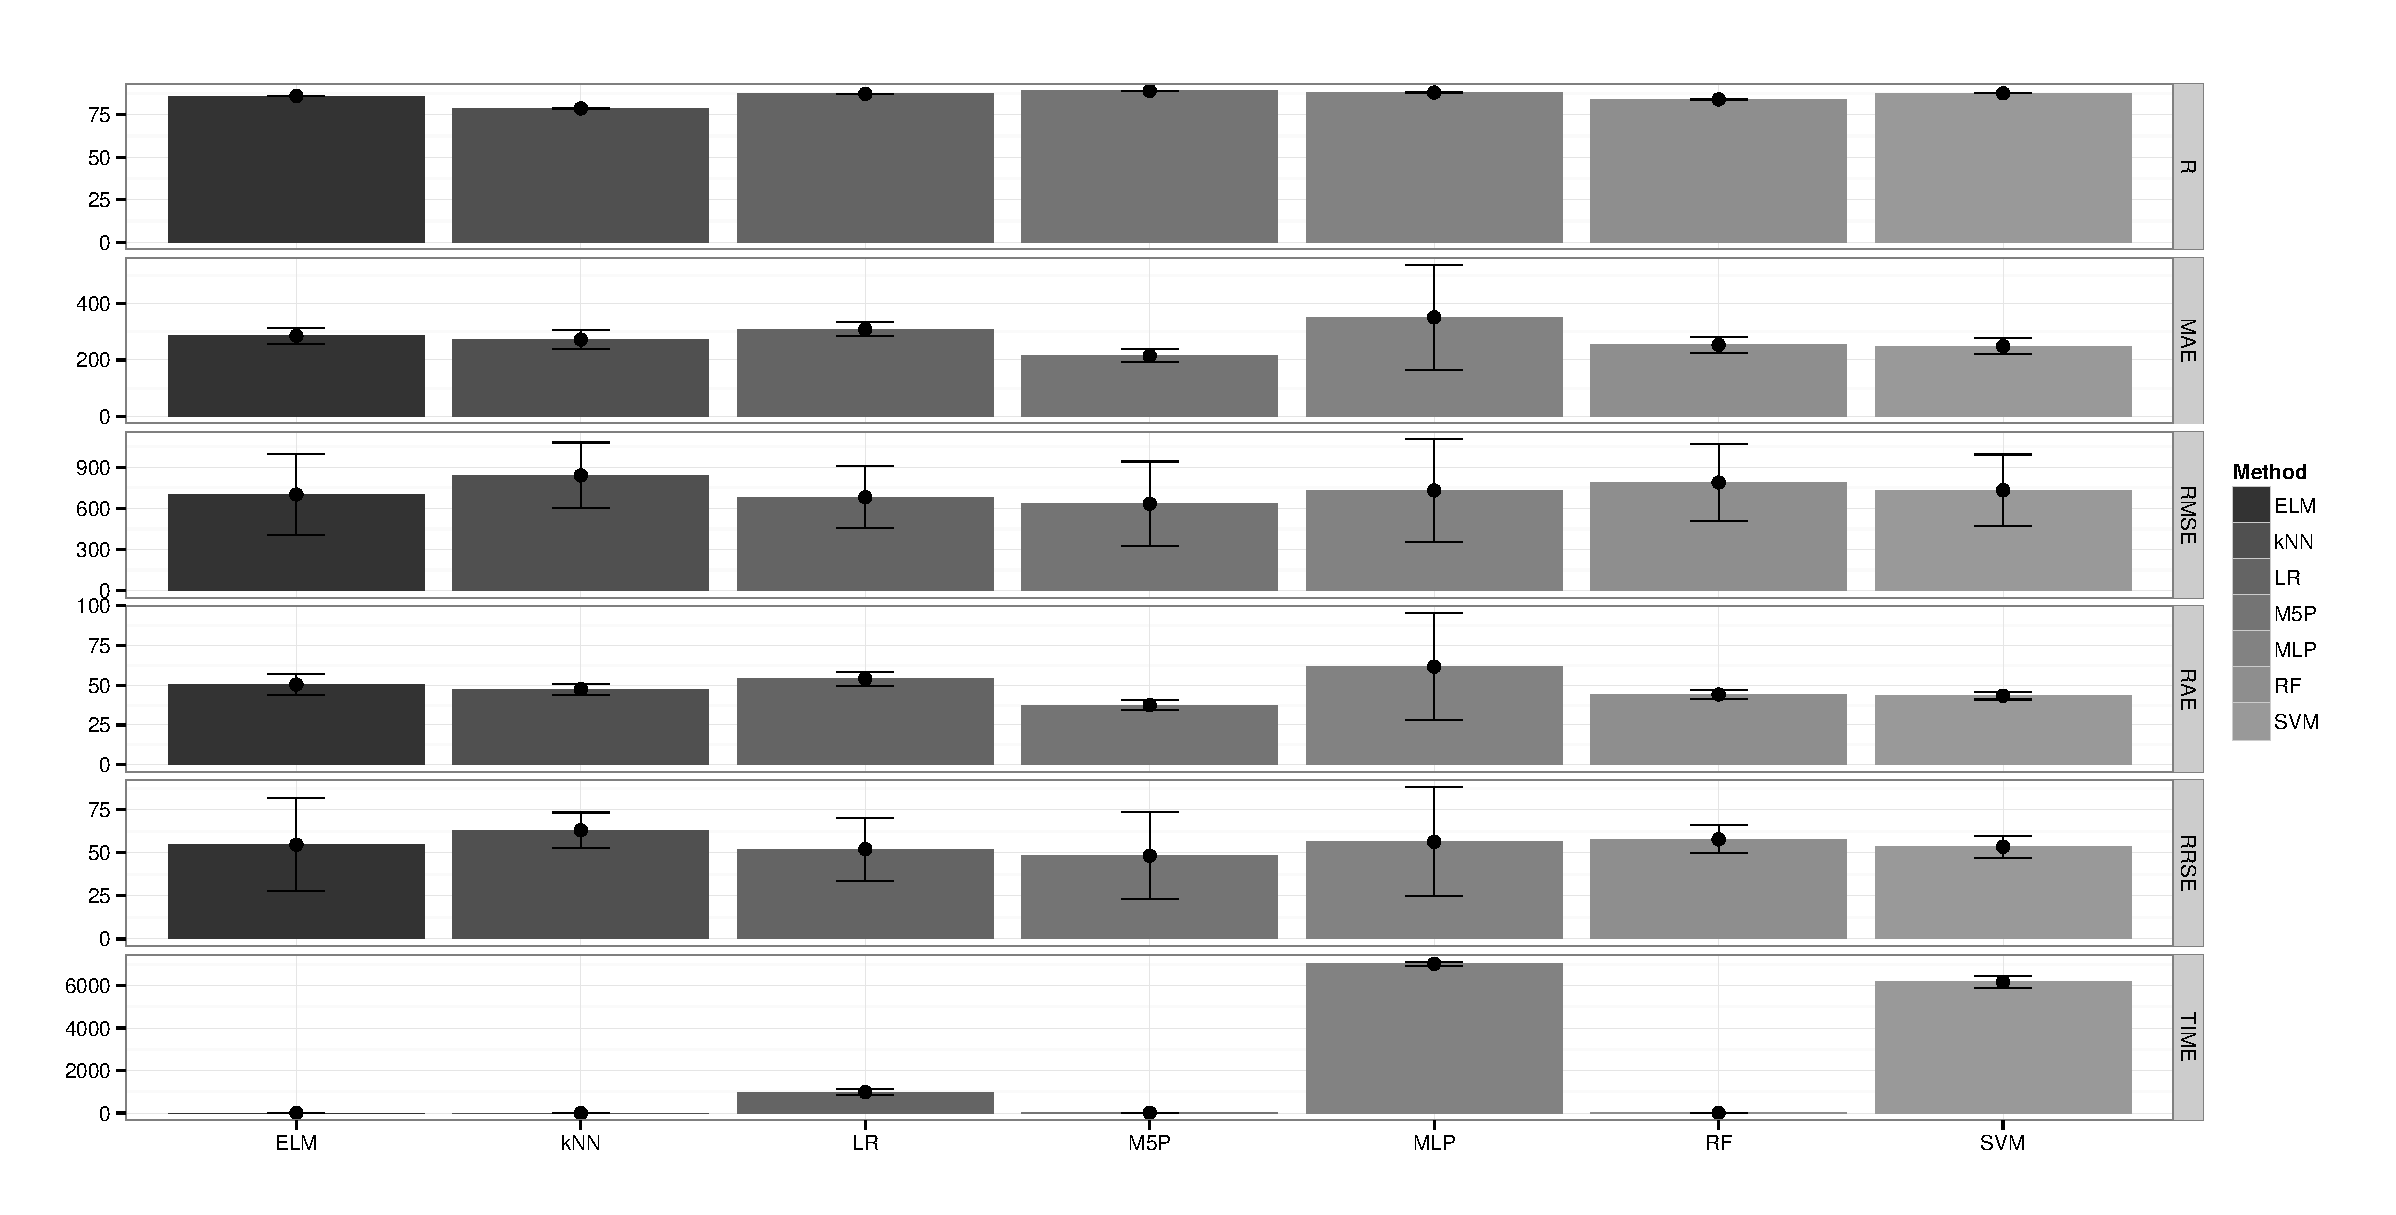
\includegraphics[scale=0.38]{./imgs/prediction_all_publisher_all_features_Table3.eps}
\end{center}
\caption{Barplots showing the values obtained predicting \texttt{total\_sales}, including errorbars, with different regression methods (30 repetitions, 10-fold cross validation). All publishers and all the features have been considered.}
% Antonio - Should we explain the meaning of the dot and the small lines in every barplot? I guess they are mean and standard deviation, aren't they?
\label{fig:all_publishers_no_fs}
\end{figure*}


As far as the different methods are concerned, M5P model obtained the best results, 
both in time and error. The advantage of M5P is that it can learn and tackle 
regression tasks that have high dimensionality and categorical variables efficiently. 
Moreover, M5P generates reproducible and comprehensible representations that 
provide information on the decision process and does not require human intervention 
either for the operation or for interpretation. Thus, it is a very suitable model to be incorporated in a publishing company processes (as we will show in 
Section \ref{subsec:decision_trees}).

Taking into account the obtained results by SVM model, this method obtains comparable errors to those of M5P. Even when using roughly tuned parameter values, it shows a good generalisation performance. However, SVM is much slower than the others to build the model, not only when using the dataset with categorical input variables, such as \texttt{collection} and \texttt{binding}, but also when using the datasets with numerical variables, not to mention the extra time needed to optimize its hyperparameters.

According to Figure \ref{fig:all_publishers_no_fs}, it can also be noticed that 
the Linear Regression model gets a better correlation value and some error measures than other complex methods like the Random Forest. 
%Although, Linear Regression is considered as a simple model to build, more powerful models can obtain better results in comparable time.  % I change this sentence as its meaning is 'strange'...  [pedro]
% Antonio - I have rewritten it. ;)
So even though Linear Regression is considered as a simple model to build, it can obtain better results than more powerful models in comparable time.

kNN is the fastest method used in this study in terms of training time, as it 
is the simplest one. However, the model is slow when classifying a large number of 
training examples, and it exhibits a poor generalisation ability since it does 
not learn enough from the training data.

%Moreover, in these experiments it has been seen the difficulty for some classifiers like the SVM to process information related to categorical variables, such as \texttt{collection} and \texttt{binding}.

MLP also gets a very good correlation coefficient. However, it takes the largest time to built the models, and obtains high error measures. ELM shows a good balance, since it is very fast in the training phase (the second fastest) and yields good results according to the correlation and the error metrics.

As a first conclusion, paying attention both to the cost in time to obtain the 
forecasting models and their accuracy, the M5P model would be the most adequate 
to solve the problem of how many books should be printed when a new book is 
published considering all the pre-sales data. Therefore, this forecasting method, with these additional advantages, can be used for products with historical sales data and for new products with little or no historical data available.

It is important to note that both RF and M5P have an embedded feature selection mechanism (the variables which compose the final trees), however this is part of their inherent procedure. In the following section we will apply three filter-based feature selection techniques on the dataset, so all the methods will profit.

%--------------------------------------------------------------------------

\subsection{Feature selection}
\label{subsec:feature_selection}

In the second stage of the experiments, different feature selection methods have been applied. The aim of these methods is to reduce the number of features considered in developing the forecasting models which consequently simplify the complexity of the models, improve their interpretability and decrease the training time. The simpler models generated after performing feature selection could give the decision maker a better insight on the underlying process by identifying the most influencing variables. 
  
We have used both the {\tt CfsSubsetEval} (CSE) \cite{Hall1998} (a correlation-based feature subset evaluation method) and the ReliefFAttributeEval (RFE) \cite{RobnikSikonja1997} (an adaptation of relief for attribute estimation) evaluation methods, implemented in the Weka tool and described in Section \ref{subsec:fs_techniques}.


\begin{figure*}[ht]
\begin{center}
\includegraphics[scale=0.35]{som_planes.eps}
\end{center}
\caption{U-matrix and component planes.}
\label{fig:componentplanes}
\end{figure*}



The dataset has also been analysed using SOM, and a visual exploration of the obtained results has been performed in order to determine the best variables to consider.
An important preprocessing step has been carried out before conducting the SOM analysis. Thus, the two categorical features \texttt{collection} and \texttt{binding} have been removed from the analysis since SOM cannot deal with them without a previous transformation into numerical ones. However, since they have a large number of unique different values this would be finally impracticable and useless. 

In the analysis, several configurations for SOM have been tested, and the best one regarding both the \textit{quantisation error} and \textit{topographic error} has been chosen. The first error is a measure which represents the average distance between every input pattern and its BMU (i.e. how good the map fits the dataset). The latter refers to the topology of the map and its preservation, so it measures an average value computed looking at both, the first and the second BMUs for every pattern. If they are neighbours (directly connected in the map) a `1' is considered, otherwise a `0' is taken. A small value would mean that the map preserves well its topology.

Thus, the chosen map to represent the data has $26 \times 16$ neurons and a hexagonal neighbourhood topology. The best SOM training results have been obtained with a final quantisation error of 0.691 and topographic error of 0.046.


Figure \ref{fig:componentplanes} shows the U-matrix along with the component 
planes analysis resulted from SOM training. The term component refers in SOM 
to a variable or feature of the problem.
The component planes in Figure \ref{fig:componentplanes} show the trend of 
values of the prototype vectors of the SOM map units. These values are represented 
as colours. The colourbar on the right of each component plane shows the indication 
of each colour. On the other side, the U-matrix on the top
left corner shows the distances between the adjacent units. It is
important to note that high values in the matrix indicate large
distance between the units of the map. It can be noticed also that
there are more hexagons in the U-matrix than component planes since
the distances between units are also represented as inter-neuron hexagons. 


\begin{table*}
\caption{Input features/variables selected by each method
\label{tab:features_selected}}
\centering{}%
{\footnotesize
\begin{tabular}{|c|c|c|c|c|}
\hline 
No. & Variable & CfsSubsetEval & ReliefFAttributeEval & SOM\\
\hline 
1 & \texttt{ret\_price} &  & $\checkmark$ & $\checkmark$\\
\hline 
2 & \texttt{subject1} & $\checkmark$ & $\checkmark$ & $\checkmark$\\
\hline 
3 &  \texttt{collection} &  &  & \\
\hline 
4 & \texttt{binding} &  &  & \\
\hline 
5 & \texttt{gifts} &  & $\checkmark$ & $\checkmark$\\
\hline 
6 & \texttt{distrib\_novelty} &  & $\checkmark$ & \\
\hline 
7 & \texttt{tot\_points\_sale} &  & $\checkmark$ & $\checkmark$\\
\hline 
8 & \texttt{tot\_points\_sale\_1st\_year} & & $\checkmark$ & \\
\hline 
9 & \texttt{weeks\_sale} &  & $\checkmark$ & $\checkmark$\\
\hline 
10 & \texttt{print\_run} & $\checkmark$ & $\checkmark$ & $\checkmark$\\
\hline 
\end{tabular}
}
\end{table*}



\begin{figure*}[ht]
\begin{center}
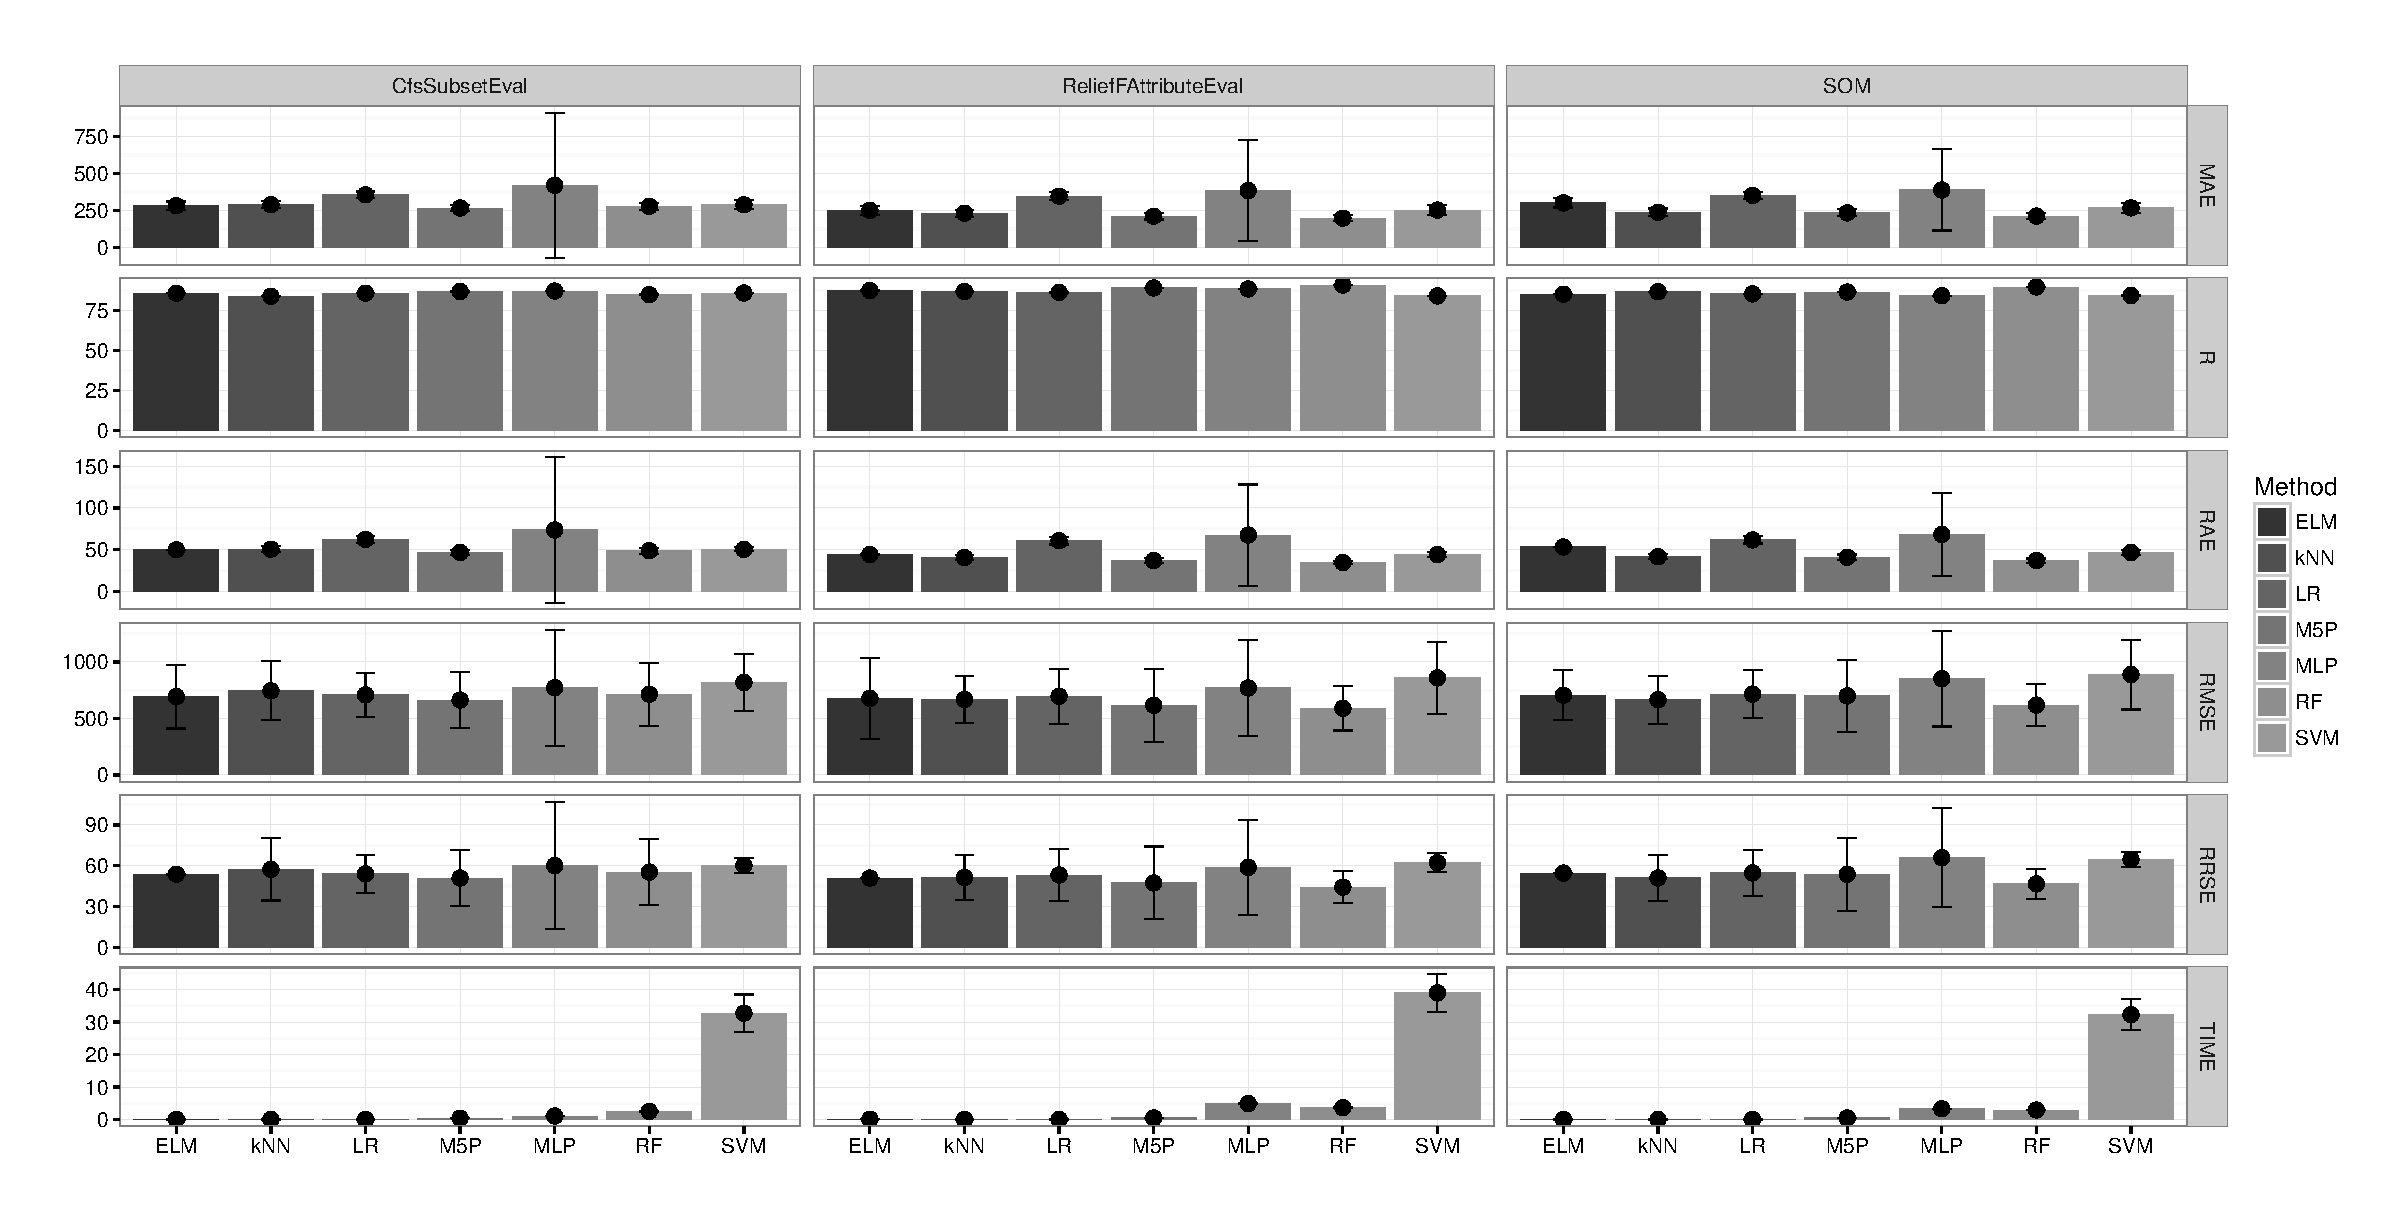
\includegraphics[scale=0.40]{./imgs/prediction_all_publisher_Table5.eps}
\end{center}
\caption{Barplots showing the values obtained predicting \texttt{total\_sales} with different regression methods (30 repetitions, 10-fold cross validation). All publishers and just those features selected by each method have been considered in every case.}
\label{fig:results_all_publishers_fs}
\end{figure*}


Examining the component planes shown in Figure \ref{fig:componentplanes}, it can be noticed that some variables have very similar colour maps which means that they are highly correlated. In this case, we have two examples; the first is the \texttt{distrib\_novelty} and \texttt{print\_run}variables while the second is the \texttt{tot\_points\_sale} and \texttt{tot\_points\_sale\_1st\_year}. In order to make the dataset having less number of uncorrelated features with each other, one of the redundant features is removed from each pair of features. Therefore, the \texttt{distrib\_novelty} and \texttt{tot\_points\_sale\_1st\_year} were omitted from the dataset.


The selected features using each one of the three methods are shown in 
Table \ref{tab:features_selected}.
Logically, just the independent or input variables are considered.



After applying the feature selection process, we have run the same
forecasting models as in Section \ref{subsec:results_all_publishers}
for the whole dataset (all the publishers), but considering only the
selected features by each method. 
The results are shown in Figure \ref{fig:results_all_publishers_fs} 
(numeric results are shown in Table \ref{tab:results_all_publishers_fs}
in the appendix of tables).
Examining the obtained results for each feature selection method, 
it can be seen that RFE got the best results in the comparison with SOM and CSE, both considering the quality/accuracy and also the standard deviation.
This could be explained due to the extensive reduction made by CSE and due to 
the `subjective' (but not so accurate) human intervention in the case of SOM. 
It can be noticed also that we obtain better results using M5P, kNN, and RF with the set of features selected by RFE than using all features, so the application of FS has improved their overall performance.

As expected, in general, all feature selection methods have reduced the training 
time needed to build the forecasting models, considerably in the most time expensive in previous experiment. This is because they reduced the 
considered features and mainly because they excluded the categorical features, 
which are the hardest to be managed (they have many possible values). 
On the other side, CSE and SOM did not perform as good as RFE. 


%********************************************************************************

\section{Experiments of special publishing companies cases}
\label{sec:example_cases}

This section presents further experiments conducted on data concerning four 
specially relevant publishing company cases. These companies were 
selected as representative cases which could be very interesting for decision 
makers and managers in the domain. The four cases are described as follows:

\begin{table*}
\caption{Description of publishing companies considered as special cases.}
\centering{}%
\resizebox{14cm}{!}{
\begin{tabular}{|c|l|l|l|}
\hline 
 Case & Different books sold & Total copies sold & Description\\
\hline 
\textit{All publishing companies} & 6083 & 3201645 & 209 publishing companies\\
\hline 
\textit{UDL929} & 216 & 460752 & Best selling publishing company\\
\hline 
\textit{UDLW12} & 97 & 2635 & Mid-range selling publishing company\\
\hline 
\textit{UDL704} & 293 & 58236 & Publishing company with most different\\ 
       &     &       & books sold\\
\hline 
\textit{UDLU11} & 180 & 249481 & Publishing company with medium number\\ 
       &     &       &  of different books sold\\
\hline 
\end{tabular}
}
\label{Table:special_cases}
\end{table*}


\begin{figure*}[ht]
\begin{center}
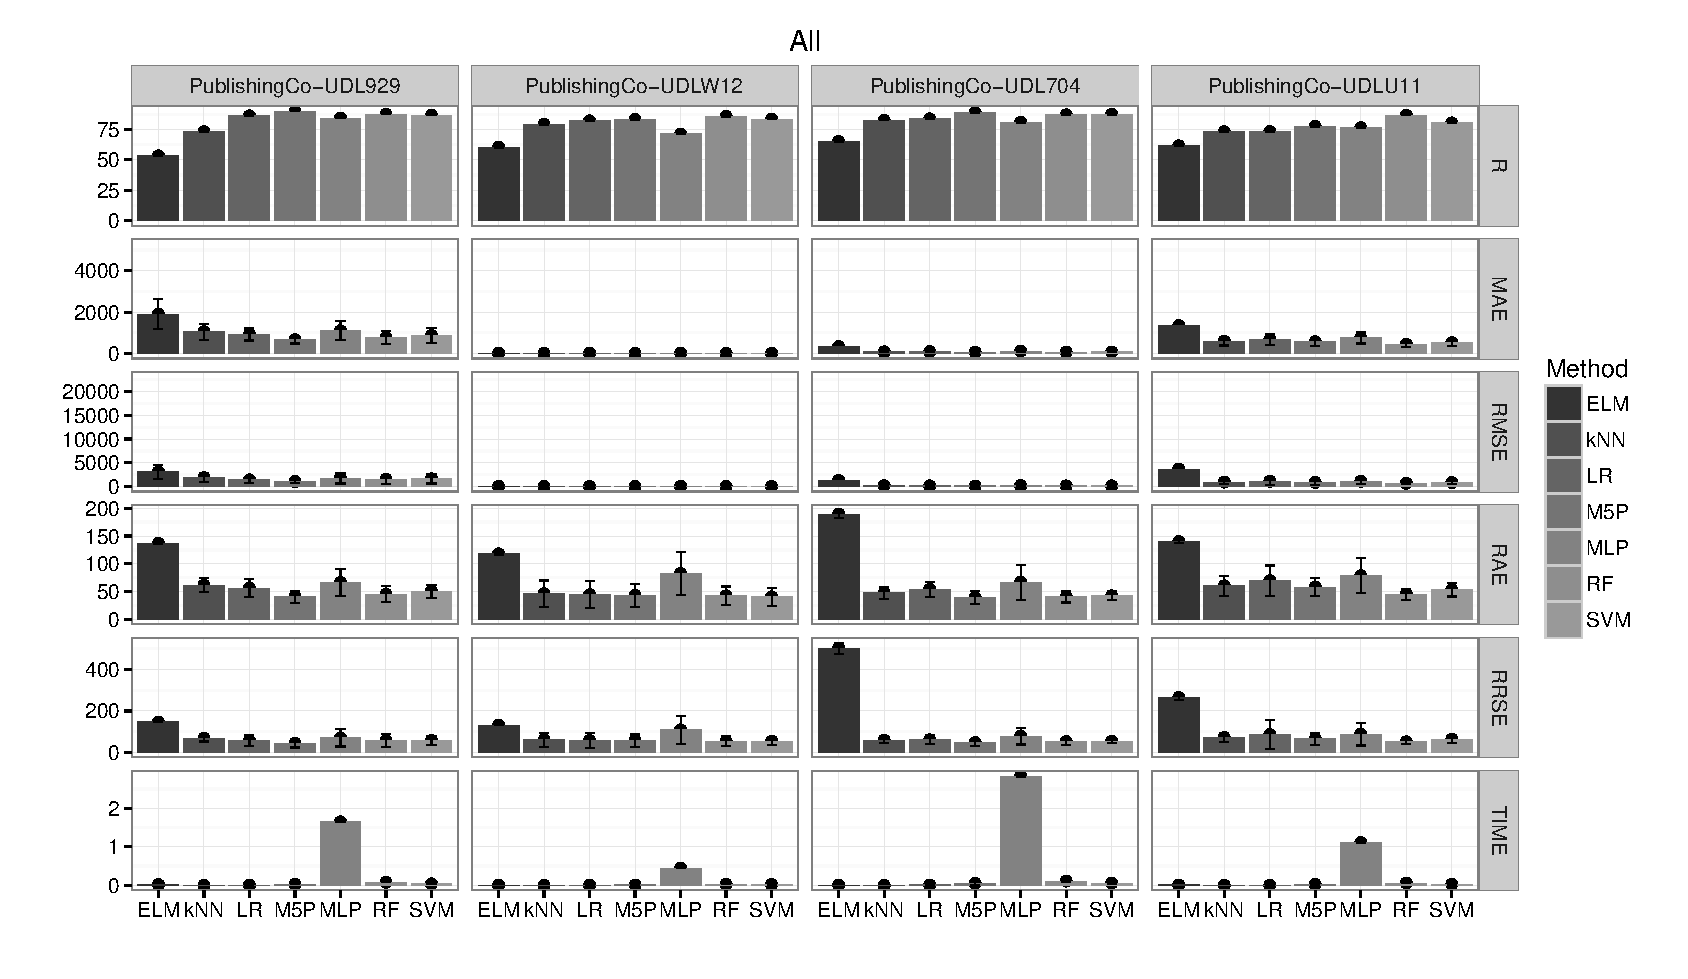
\includegraphics[scale=0.58]{./imgs/attribute_All.eps}
\end{center}
\caption{Barplots showing the values obtained predicting
  \texttt{total\_sales}, using all features, with different regression
  methods (30 repetitions, 10-fold cross validation). Results obtained
  for different special publishing companies: UDL929 (the best selling
  publishing company), UDLW12 (the median selling publishing company),
  UDL704 (highest number of different titles sold) and UDLU11 (medium
  number of different books sold). 
}
\label{fig:attributeAll}
\end{figure*}

\begin{itemize}
    \item \textit{Best seller publishing company}: this case represents the publishing company that sells the highest number of copies regardless the title of the books sold. Therefore, it is an example of a case on a higher business scale.
    \item \textit{Mid-range seller publishing company}: this represents a publishing company that sells medium number of copies compared to other publishing companies (Medium business scale). 
    \item \textit{Highest variation publishing company}: this is an example of a publishing company that follows a strategy in publishing a very wide range of different titles.
    \item \textit{Medium varied publishing company}: this case represents a publishing company that has a median rank between the other publishing companies regarding the variety of titles sold.
\end{itemize}


Table \ref{Table:special_cases} shows the number of sold copies and the number 
of titles published by the selected companies.



The experiments applied on the selected special cases follow the same methodology used previously for the whole dataset. First, the forecasting models are applied on each dataset using all features, then, the three feature selection methods (RFE, CSE and SOM) are used to reduce the set of features in each case. Second, the regression models are applied again on the reduced datasets to evaluate their performance.

Evaluation results of the obtained models (without performing any feature selection method) for the selected four cases have been summarized in Figure \ref{fig:attributeAll} 
(numeric results can be seen in Tables 
\ref{Table:case1results_no_fs}, \ref{Table:case2results_no_fs}, 
\ref{Table:case3results_no_fs} and \ref{Table:case4results_no_fs} 
in the appendix of tables).

Results in the figure show that the models performed similarly to the case of 
the global models for all publishers, which were previously presented in 
Figure \ref{fig:all_publishers_no_fs}. 
In general, M5P, RF and SVM performed better than the `simple' classifiers kNN and LR, and also better than MLP and ELM. Actually, the latter presents a low performance in these special cases (not previously for the whole dataset).
This could be due to the reported low robustness of the basic ELM version \cite{ding2015deep}, which we have applied in this work. More advanced versions such as the Multi-layer ELM, Hierarchical ELM and ELM with kernels will be investigated and experimented in the future work in order to reach better generalization performance.

In the case of Best selling publisher houses (i.e. UDL929) and publishers who 
publish a wide range of different books (i.e. UDL704), M5P could be recommended 
as it shows more accurate forecasting results than the other models. 
While in the case of medium sized publishers, in terms of sales and number 
of published books, the RF model would be adequate.


%--------------------------------------------------------------------------
%\subsection{Sales forecasting with feature selection}
%\label{subsec:case_sales_feature_selection}

Now the feature selection methods (RFE, CSE and SOM) are applied in each case
independently, since publishers with different sales ranges, and targets, might in fact include different factors or have different leverage when deciding how much to print. 

%  esta frase siguiente ya no, ya que además de pasar las tablas al apéndice, vamos a mostrar la figura:
%For clarity purpose, obtained results after applying feature selection methods have been shown in Tables \ref{Table:case1results_no_fs} to \ref{Table:case4results_fs_som} in the appendix of tables at the end of this paper. In those tables it can be seen that, as in the previous experiment, the highest predictive power is exhibited by RFE over CSE and SOM feature selection methods. In this sense, RFE reduction has noticeably improved the performance of all models, specially in the case of the best selling publisher house (i.e. UDL929) and the publisher which publishes a wide range of different books (i.e. UDL704). 

%  esta frase siguiente ya no, porque vamos a pasar las tablas al apéndice
%For clarity purpose, we present here only the results after applying the RFE method for the four cases in Tables \ref{Table:case1results_fs_rf}, \ref{Table:case2results_fs_rf}, \ref{Table:case4results_fs_rf} and \ref{Table:case4results_fs_rf}, this one was chosen since the selected features by this method showed in the previous experiment the highest predictive power among  all classifiers. RFE reduction has noticeably improved the performance of all classifiers specially in the case of the best selling publisher house (i.e. UDL929) and the publisher which publishes a wide range of different books (i.e. UDL704). For the rest of the results which are obtained by CSE and SOM feature selection methods we refer the reader to the appendix of tables at the end of this paper.

For clarity purposes, only obtained results after applying the RFE method for the 
four cases are shown in Figure \ref{fig:casesReliefFAttributeEval}.
Detailed numeric results of RFE on the special cases can be seen in 
Tables \ref{Table:case1results_fs_rf}, \ref{Table:case2results_fs_rf}, 
\ref{Table:case3results_fs_rf} and \ref{Table:case4results_fs_rf}
in the appendix of tables. 
RFE was chosen since the selected features by this method showed in the experiment with the whole dataset the highest predictive power among all models.
For the rest of the results which are obtained by CSE and SOM FS methods, we refer the reader also to the appendix of tables.

As it can be seen, RFE reduction has noticeably improved the performance of all 
classifiers specially in the case of the best selling publisher house (i.e. UDL929) and the one which publishes a wide range of different books (i.e. UDL704). 

\begin{figure*}[ht]
\begin{center}
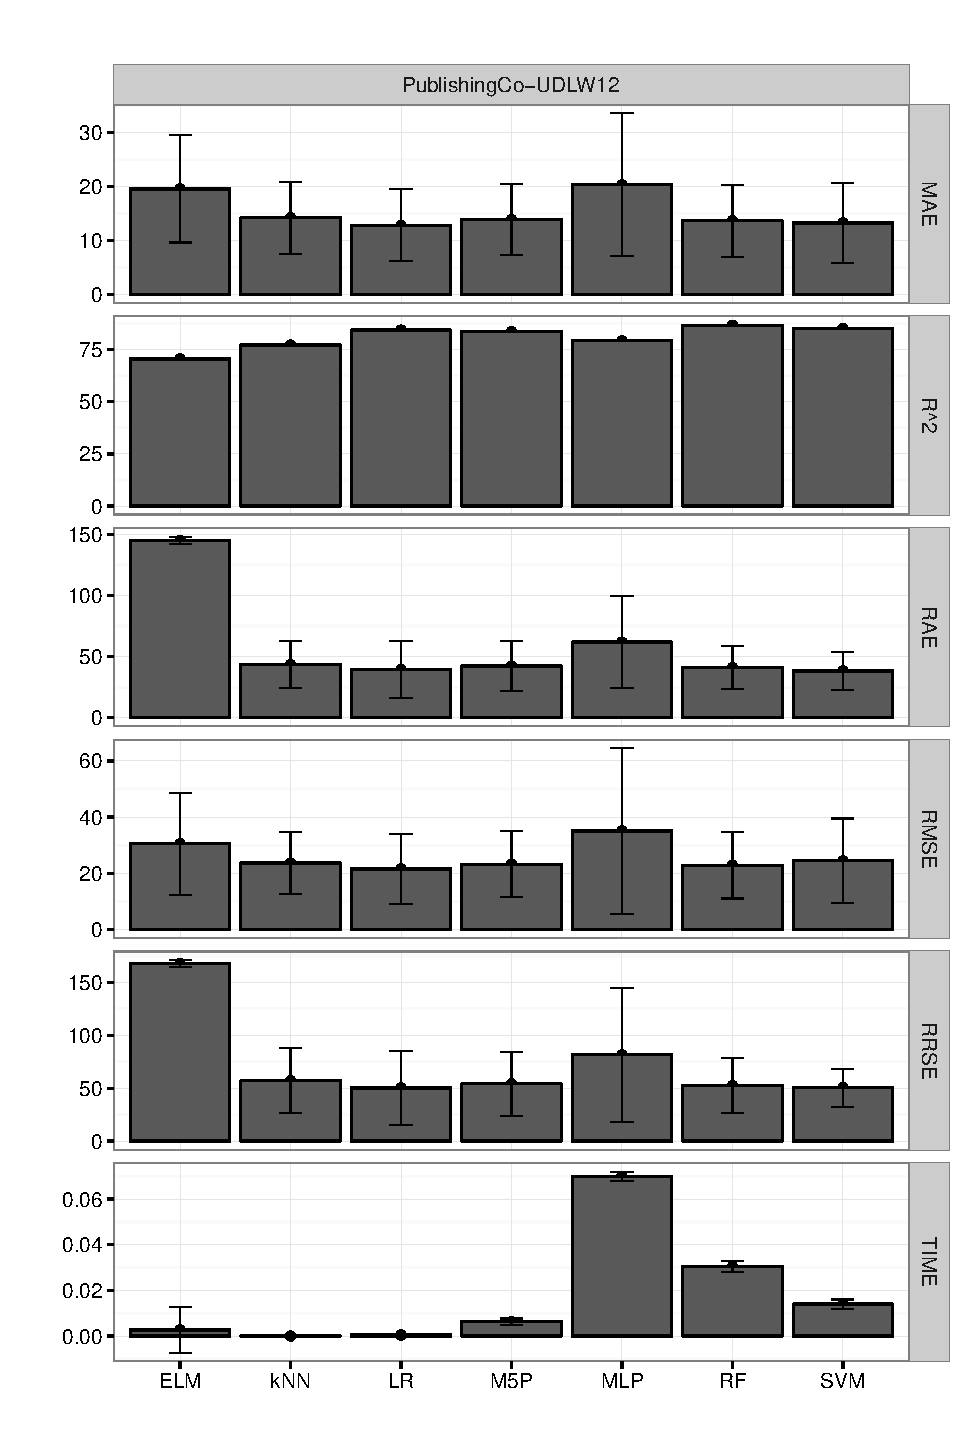
\includegraphics[scale=0.58]{./imgs/attribute_ReliefFAttributeEval-FS.eps}
\end{center}
\caption{Barplots showing the values obtained predicting \texttt{total\_sales}, considering just the features selected by ReliefFAttributeEval method, with different regression methods (30 repetitions, 10-fold cross validation). Results obtained for different special publishing companies: UDL929 (the best selling publishing company), UDLW12 (the median selling publishing company), UDL704 (highest number of different titles sold) and UDLU11 (medium number of different books sold).
}
\label{fig:casesReliefFAttributeEval}
\end{figure*}


%--------------------------------------------------------------------------

\subsection{Case study: publisher with the most sales}
\label{subsec:decision_trees}

What is, then, the model obtained by our method? What factors have
the biggest influence in sales and how can a publisher use them to gauge
sales of a new book? In order to do that, we have examined the models
built during the regression. Namely, we present two of the decision
trees generated by M5P method applied to the data of the publisher
that sells the most. By looking at these trees, the publisher should
be able to decide how many actual books should be printed to put them
for sale, which was the initial objective of our research.

The model obtained for the publishing company UDL929 is shown in
Figure \ref{fig:decision_tree_best_seller}, which was the company that
sold the most books in our dataset. It makes sense to use data for a
single company, since book sales for all companies is only available
if you buy it; a single company, however, will have complete data on
its own sales. This company is also representative because, being the
one that sells the most, it will have the biggest range of sales for
individual books. In this figure, tree {\em leaves} correspond to
linear regression models that can be easily computed to obtain the
final predicted value for book sales.
The second decision tree (Figure
\ref{fig:decision_tree_best_seller_fs}) corresponds to the same
publishing company, so the same data were used, but the RFE %ReliefFAttributeEval
feature selection method was applied. This simplification, besides making the
tree easier to understand, reduces training time to a fraction of what
was needed before the selection method was applied. 

Examining both trees, it can be noticed that
\texttt{tot\_points\_sale} variable appears twice in the trees, being also the root
% I'm reducing some paragraphs by eliminating some sentences that appears repeated.
(it has the biggest influence on the decision models and also a major role in forecasting the total sales, implying that the books have to physically {\em be} in the point of sale).
% This indicates that the total number of points of sale has the biggest influence on the decision models and also a major role in forecasting the total sales, implying that buyers have to actually {\em see}, maybe browse the book, before buying it. Books have to physically {\em be} in the point of sale, so this number gives a lower bound to the number of books that have to be printed; a stack of book will have to be present in each point of sale to attain that effect. 
This is an interesting clue for the
experts, who could check the expected impact of different number of
selling points. This feature also shows that there are different
regimes depending on the number of points of sale, with best sellers
being those that are distributed to more than roughly 500 points. 


\begin{figure*}[!ht] 
\begin{center}
  \epsfig{file=decision_tree_no_fs.eps,width=13cm}
\caption{Decision tree built by the M5P method for the best seller publishing 
	company including all pre-sales features.}
\label{fig:decision_tree_best_seller}
\end{center}
\end{figure*}

\begin{figure*}[!ht] 
\begin{center}
  \epsfig{file=decision_tree_fs.eps,width=13cm}
\caption{Decision tree built by the M5P method for the best seller
  publishing company using the subset of features selected by the
  {\sf ReliefFAttributeEval} method.} 
\label{fig:decision_tree_best_seller_fs}
\end{center}
\end{figure*}

The second {\em splitting} feature, number of books distributed as a
novelty, gives the publisher a hint on how many books have to be sent
to bookstores to stack on the {\em novelty} table. You need to sell
roughly 5, the result of dividing 2807.5 and 550.5, to have a lower
bound in sales at 1006, which is negatively impacted by the retail
price and the number of points of sale in the first year of
distribution. In all cases, the last number in the formula featured in
the box gives you a baseline for sales, which the rest of the
variables impacting positively or negatively. A whole treatise could
be written on this decision tree, but in this case, let us look a bit
more closely at this box and try and interpret it. For instance, the price
in this case will impact negatively on sales. For a typical retail
price of a trade paperback of 12 euro, we would be looking at negative
sales (if we disregard the rest of the variables), which in this case
will indicate that these are the kind of books, maybe paperbacks, that
sell for a low price of around 5 euro. You also have to look at the
relation between the factor for total points of sale and the total
point of sales the first year. The fact that this last one is bigger
indicates that the publisher will have to {\em increase} the number of
points of sale after the first year, distributing it more shops at a
more capillary level; the number of points of sale will have to be
increased by 10\% to achieve a bit more than the baseline. All in all,
the conclusion with this part of the tree is that you will have to
print around 3000 books to sell a quantity that will start at 1000,
one third of the print run, and changes depending on a number of
factors, including price.

The right hand side of the tree includes those books that are
distributed in a bigger percentage of the total amount of point of
sale available in Spain, which in Spain includes not only proper
bookstores, but also press stands and even supermarkets and hovers
around several tens of thousands (around 24000, according to
\cite{POS}), so we are clearly talking best sellers here distributed in
as many places as possible. The first tree
(in Figure \ref{fig:decision_tree_best_seller}) gives an idea of what we
are talking about, sales start at 1000 but the single factor that has
a bigger influence on sales is the topic, which has to be either 23 or
1. `1' is the first digit of the classification used for all kinds of
general literary books. `23' includes philology, which includes either
textbooks of maybe books in a foreign language; there are just a few
of those, with `1' being far more common. So, in principle these would
be the typical best-sellers, literary prizes and big hits, but we
would have to look more closely at the second tree
(in Figure \ref{fig:decision_tree_best_seller_fs}) to check what are other factors
influencing sales. It is also interesting that the number of total
points of sale comes multiplied by 7, which would be a good baseline
of books sold per outlet and give the publisher with a ballpark,
around 4000 books, to print in the first print run. The picture
painted by the second tree is a bit more bleak; obviously, even big
publishing house produces flops from time to time, and those would be
books which eventually print less than around 12500, indicating that
there has not been a second print run, since best-seller print runs
used to start at 15000 books\footnote{Nowadays in Spain that number
 would be closer to 5000}. In general, that branch of the tree paints
a pretty bleak picture: no matter how you combine the variable values,
it will end up with sales much lower than the print run. The main
problem with this tree is that its predictive value, with the
variables that we have, is not too high, except for the hint we have
on the subject matter. At the end of the day, there is a certain
amount of unpredictability in how much a book sells and the only
information we can give the publisher if he finds books sales adapt to
this model is to boost points of sale and lower price so that sales
pick a bit; in this sense and in certain cases, our model is more
informative than predictive, but having numeric models helps anyway
the publisher with tailoring print runs and even increasing sales of
books that have been already printed.

The last box on the right of Figure
\ref{fig:decision_tree_best_seller_fs} has a negative baseline, but
this only indicates that the influence of the print run will be
bigger. This probably indicates books that have been reprinted due to
demand and it also tells how many are sold in every outlet: around 29
books. The price, number of initial points of sale, number of books
distributed as novelty and gifts all have a negative factor, but this
is related to the fact that they will have to be selling for a long
time, that is, not only be better, but also long sellers, which is also
indicated by the positive factor in the number of weeks they are for
sale. 

All in all, these seven groups revealed by the tree in Figure
\ref{fig:decision_tree_best_seller_fs} constitute not only an accurate
model for predicting book sales based on data available to the
publisher, but also an informative tool that will allow publishers to
estimate print runs based on forecasted sales, and establish other
factors such as price, number of points of sale, and number of books
distributed to outlets. 

An important fact that these tree models reveal is that marketing
variables, such as the total number of points of sale and the number
of units distributed as novelty have higher influence on the
prediction than the selling price of the book, which could be,
initially, considered as one of the most important parameters to
determine sales. This interpretation leads us to suggest that
companies could probably improve the accuracy of their sales
forecasting models by incorporating more marketing related variables
in their models. This does not mean that the retail price is not a
factor; it appears on all models, but it will be a secondary factor
that will have to be decided once the main ones are settled. 


%********************************************************************************
\section{Conclusions and Future Work}
\label{sec:conclusionsAndFutureWork}

In this paper, the problem of 
predicting total sales in order to print the right amount of books
%how many books should be printed 
when a new book is going to be published is faced using several data-mining 
and forecasting methods.

This is a very challenging problem in this industry, because printing
a much higher 
number of volumes than those finally sold will lead to losses, while
printing an adequate number of copies will optimise sales and company
earnings.  
In addition, there are several difficulties inherent to the new book
sales forecasting, such as the limited amount of historical data to
consider or the variability of the market (fashions, seasonality),
which do a difficult task finding an adequate forecasting method. 

A dataset consisting of 6000 books provided by the Spanish publishing
company Trevenque Editorial S.L. has been used. This data has been
analysed by means of Self-Organizing Maps as a visualisation tool, and
two other Feature Selection techniques, namely a correlation-based
feature subset evaluation method, and an adaptation of relief for
attribute estimation. Using these methods the most relevant variables
when predicting sales have been determined, while unrelated or
superfluous ones have been removed. 

Four different datasets have also been extracted from the original
one, each one corresponding to a publishing house which we have
considered as representative: the one with the most number of sales,
the one with the medium number of sales, with the most varied sales
(different books), and with a medium number of different books sold. 

Considering these datasets and the complete one, five machine learning
models for sales forecasting have been configured (according to the
problem requirements) and used to predict new book sales, from which
the optimal print run could be estimated. These algorithms include
some based on Decision Trees (M5P and Random Forest), kNN, Support
Vector Machines and Linear Regression. 
These methods have been evaluated considering several performance
indicators (error measures) and also the time consumed to build the
corresponding models. 

As a conclusion, M5P yields the best results overall, obtaining the best accuracy 
(lowest error) on average, even with acceptable values regarding the training time.
In addition, the Decision Trees obtained with this method have been
shown to be an excellent decision-aid tool for publishers, since they are accurate 
and quite easy to understand and apply. 
They are also able to provide insights on the decision variables that
have a higher influence on the predicted sales for these publishers. 

This, compared to the output of black-box models such as artificial
neural networks, was a determining advantage from the point of view of
the needs of experts and the company that initially contacted us for
this work. 

The feature selection techniques have also shown to positively affect
all the results, yielding a better performance in time to train while
maintaining good accuracy. Moreover, their application leads to obtain
even simpler models. 

Overall, this study contributes to the literature by proposing the use
of different soft-computing standard techniques to solve a new
challenging problem. 
Moreover, proposed method, consisting in selecting features and
applying different models for different types of publishers could be
implemented, not only in the publishing  
industry, but also in other domains where the specificity of products
is similar such as novelty items or toys, and might be of interest to other 
academic researchers and industrial practitioners.

% -------- Future Work ---------

As future work, it would be interesting to compare the obtained
forecasting results with those yielded by other soft-computing
methods, such as genetic programming, recommend systems or fuzzy logic. 
Moreover, even if the methods have been configured to obtain the best
forecasting results, it would be of interest carrying out some
automatic parameter-tuning procedure by means of optimisation
meta-algorithms \cite{huang2006ga,Mookiah2013_EA_Tuning,Shen2016_FFly_Tuning}, 
for instance. 

In addition, if data for other countries were available, it would be
interesting to observe, and factor in the method, country differences,
even considering the same book and how it is sold in different
countries. 

Furthermore, since there are some characteristics that may affect product sales 
significantly, another way to improve sales predictions could be making a 
thorough study of the effect of the application of discounts and promotions. 

Finally, there are some variables over which the publisher has some
control once the book has been published, such as the initial print run, 
the books offered as gifts to reviewers, or what proportion is going to be sent 
to each possible point of sale. These can be incorporated into an optimisation 
model that will optimise those values to obtain desired sales. 


%********************************************************************************
\section*{Acknowledgements}

This work has been supported in part by projects PreTEL (PRM Consultores - Trevenque S.L.), TIN2014-56494-C4-3-P and TEC2015-68752 (Spanish Ministry of Economy and Competitiveness and FEDER), PRY142/14 (Fundaci{\'o}n P{\'u}blica Andaluza Centro de Estudios Andaluces en la IX Convocatoria de Proyectos de Investigaci{\'o}n), and PROY-PP2015-06 (Plan Propio 2015, funded by the University of Granada, Spain).


%********************************************************************************
\bibliographystyle{elsarticle-num}
\bibliography{refs}
% TODO:
% the final list of references should be imported here from the .bbl file 
% obtained after compiling the main LaTeX file.
% And the previous line (\bibliography{refs}) has then to be commented.

%----------------------------------------------------------------------

\newpage
\clearpage
\onecolumn

\appendix
\section{APPENDIX TABLES}

% ----------------------- Tables in the Appendix---------------------------

%--------------- old Tables 3, 5 (before revision)

\begin{table}[!ht]
\caption{Predicting \texttt{total\_sales} for all publishers (all the features). 30 repetitions, 10-fold cross validation. Best values in bold.
\label{tab:all_publishers_no_fs}}
\centering{}%
\scalebox{0.78}{

\begin{tabular}{|c|l|l|l|l|l|l|}
\hline 
 & $R$  & MAE  & RMSE  & RAE (\%)  & RRSE (\%)  & Time (s)\tabularnewline
\hline 
M5P  &  \textbf{89.0 $\pm$ 0.09}  &  \textbf{214.37 $\pm$ 22.96}  &  \textbf{634.23 $\pm$ 307.76}  &  \textbf{37.46 $\pm$ 3.12}  &  \textbf{48.32 $\pm$ 25.16} & 18.85 $\pm$ 0.61\tabularnewline
\hline 
kNN  & 78.7 $\pm$ 0.08  & 272.29 $\pm$ 32.38  & 840.59 $\pm$ 240.11  & 47.48 $\pm$ 3.39  & 63.07 $\pm$ 10.29  &  \textbf{0.001 $\pm$ 0.01}\tabularnewline
\hline 
RF & 84.0 $\pm$ 0.05  & 253.37 $\pm$ 29.43  & 788.94 $\pm$ 282.01  & 44.16 $\pm$ 2.76  & 57.77 $\pm$ 8.15  & 4.91 $\pm$ 0.12\tabularnewline
\hline 
LR & 87.2 $\pm$ 0.07  & 308.68 $\pm$ 25.44  & 680.91 $\pm$ 226.41  & 54.05 $\pm$ 4.38  & 52.13 $\pm$ 18.29  & 984.68 $\pm$ 128.21\tabularnewline
\hline 
SVM  & 87.6 $\pm$ 0.04  & 248.76 $\pm$ 27.49  & 732.64 $\pm$ 260.56  & 43.37 $\pm$ 2.35  & 53.47 $\pm$ 6.29  & 6169.24 $\pm$ 281.49\tabularnewline
\hline 
MLP	& 88.01 $\pm$ 0.11	& 350.99 $\pm$ 185.53	& 730.93 $\pm$ 374.84	& 61.64 $\pm$ 33.61	& 56.33 $\pm$ 31.6	& 7014.06 $\pm$ 110.095 \tabularnewline
\hline 
ELM & 	85.97	 $\pm$ 	0.11	 & 	285.64	 $\pm$ 	28.44	 & 	701.65	 $\pm$ 	293.66	 & 	50.41	 $\pm$ 	6.4	 & 	54.7	 $\pm$ 	26.93	 & 	0.1939	 $\pm$ 	0.004 \tabularnewline


\hline 
\end{tabular}
}
\end{table}


\begin{table}[!ht]
\centering{}%
\caption{Predicting \texttt{total\_sales} for all publishers based on features selected by each method. Best values in bold.
\label{tab:results_all_publishers_fs}}
% CFSSUBEVAL
\resizebox{12cm}{!}{
\begin{tabular}{|c|c|c|c|c|c|c|}
\hline 
\multicolumn{7}{|c|}{\textit{CfsSubsetEval}}\\
\hline
 & $R$  & MAE & RMSE & RAE (\%) & RRSE (\%) & Time (s)\\
\hline 
M5P &  \textbf{87.0 $\pm$0.09} &  \textbf{266.78 $\pm$23.12} &  \textbf{662.32 $\pm$245.27} &  \textbf{46.66 $\pm$3.25} &  \textbf{50.9 $\pm$20.35} & 0.41 $\pm$0.04\\
\hline 
kNN & 84.0 $\pm$0.10 & 289.09 $\pm$22.83 & 743.92 $\pm$260.45 & 50.59 $\pm$3.50 & 57.30 $\pm$22.90 &  \textbf{0.001 $\pm$0.001}\\
\hline 
RF & 85.0 $\pm$0.11 & 278.42 $\pm$23.07 & 714.13 $\pm$278.65 & 48.71 $\pm$3.43 & 55.26 $\pm$24.41 & 2.48 $\pm$0.13\\
\hline 
LR & 85.9 $\pm$0.06 & 356.35 $\pm$22.43 & 708.06 $\pm$195.15 & 62.42 $\pm$4.22 & 53.97 $\pm$14.05 & 0.01 $\pm$0.001\\
\hline 
SVM & 86.0 $\pm$0.06 & 288.47 $\pm$30.32 & 817.56 $\pm$253.24 & 50.30 $\pm$2.38 & 60.27 $\pm$5.68 & 32.73 $\pm$5.74\\
\hline
MLP	& 87.26 $\pm$ 0.1	& 420.02 $\pm$ 491.51	& 771.6 $\pm$ 514.03	& 73.6 $\pm$ 87.04	& 60.09 $\pm$ 46.83	& 1.08 $\pm$ 0.019\\
\hline
ELM & 	86.84	 $\pm$ 	0.09	 & 	283.07	 $\pm$ 	30.78	 & 	686.05	 $\pm$ 	278.37	 & 	49.88	 $\pm$ 	6.15	 & 	52.08	 $\pm$ 	20.64	 & 	0.0133	 $\pm$ 	0.003\\
\hline
\end{tabular}
}
% RELIEFFATTRIBUTEEVAL
\resizebox{12cm}{!}{
\begin{tabular}{|c|c|c|c|c|c|c|}
\hline 
\multicolumn{7}{|c|}{\textit{ReliefFAttributeEval}}\\
\hline 
 & $R$  & MAE & RMSE & RAE (\%) & RRSE (\%) & Time (s)\\
\hline 
M5P & 89.2 $\pm$0.10 & 211.15 $\pm$22.41 & 616.35 $\pm$321.25 & 36.93 $\pm$3.41 & 47.30 $\pm$26.83 & 0.49 $\pm$0.02\\
\hline 
kNN & 86.9 $\pm$0.09 & 231.78 $\pm$24.25 & 668.03 $\pm$205.14 & 40.48 $\pm$3.06 & 51.28 $\pm$16.81 &  \textbf{0.002 $\pm$0.004}\\
\hline 
RF &  \textbf{91.0 $\pm$0.05} &  \textbf{198.16 $\pm$19.50} &  \textbf{589.35 $\pm$195.80} &  \textbf{34.61 $\pm$2.27} &  \textbf{44.21 $\pm$11.63} & 3.63 $\pm$0.20\\
\hline 
LR & 86.4 $\pm$0.08 & 346.88 $\pm$25.40 & 695.90 $\pm$242.49 & 60.75 $\pm$4.55 & 53.16 $\pm$19.43 & 0.01 $\pm$0.01\\
\hline 
SVM & 84.2 $\pm$0.04 & 252.87 $\pm$33.38 & 858.26 $\pm$318.23 & 44.01 $\pm$3.04 & 62.22 $\pm$7.15 & 38.97 $\pm$5.75\\
\hline  
MLP	& 88.58 $\pm$ 0.09	& 384.94 $\pm$ 342.05	& 769.74 $\pm$ 427.35	& 67.47 $\pm$ 60.6	& 58.71 $\pm$ 34.81	& 4.9 $\pm$ 0.047\\
\hline  
ELM & 	87.25	 $\pm$ 	0.1	 & 	277.38	 $\pm$ 	27.54	 & 	669.29	 $\pm$ 	307.31	 & 	49	 $\pm$ 	6.59	 & 	51.81	 $\pm$ 	25.4	 & 	0.0677	 $\pm$ 	0.002\\
\hline

\end{tabular}
}
% SOM
\centering{}% SOM
\resizebox{12cm}{!}{
\begin{tabular}{|c|c|c|c|c|c|c|}
\hline 
\multicolumn{7}{|c|}{\textit{SOM}}\tabularnewline
\hline 
 &  $R$  & MAE  & RMSE  & RAE (\%)  & RRSE (\%)  & Time (s)\tabularnewline
\hline 
M5P  & 86.6 $\pm$0.10  & 234.09 $\pm$23.19  & 699.56 $\pm$317.20  & 40.92 $\pm$3.25  & 53.70 $\pm$26.87  & 0.475 $\pm$0.12\tabularnewline
\hline 
kNN  & 86.8 $\pm$0.09  & 237.91 $\pm$25.34  & 665.64 $\pm$212.05  & 41.55 $\pm$3.14  & 50.96 $\pm$16.72  &  \textbf{0.001 $\pm$0.004}\tabularnewline
\hline 
RF &  \textbf{89.8 $\pm$0.05}  &  \textbf{211.87 $\pm$20.07}  &  \textbf{617.78 $\pm$187.16}  &  \textbf{37.02 $\pm$2.46}  &  \textbf{46.58 $\pm$11.14}  & 2.93 $\pm$0.11\tabularnewline
\hline 
LR  & 85.5 $\pm$0.08  & 351.99 $\pm$23.72  & 714.76 $\pm$214.21  & 61.65 $\pm$4.28  & 54.67 $\pm$16.88  & 0.01 $\pm$0.01\tabularnewline
\hline 
SVM  & 84.5 $\pm$0.04  & 267.71 $\pm$33.82  & 888.33 $\pm$308.93  & 46.60 $\pm$2.87  & 64.62 $\pm$5.45  & 32.27 $\pm$4.74\tabularnewline
\hline 
MLP	& 84.3 $\pm$ 0.12	& 388.79 $\pm$ 274.18	& 851.01 $\pm$ 422.03	& 68.26 $\pm$ 49.64	& 65.85 $\pm$ 36.49	& 3.29 $\pm$ 0.042\tabularnewline
\hline
ELM & 	85.82	 $\pm$ 	0.08	 & 	299.48	 $\pm$ 	34.26	 & 	697.84	 $\pm$ 	229.85	 & 	52.78	 $\pm$ 	6.55	 & 	54.19	 $\pm$ 	19.44	 & 	0.0406	 $\pm$ 	0.003\\
\hline
\end{tabular}
}
\end{table}


% Antonio - I have reordered the tables correctly. ;D
% thanks!!! (again)  

%--------------- old Table 7 (before revision)
\begin{table}[!ht]
\caption{Predicting \texttt{total\_sales} for publishing company UDL929 (the best selling publishing company). Best values in bold. 
\label{Table:case1results_no_fs}}
\centering{}%
\resizebox{12cm}{!}{
\begin{tabular}{|c|c|c|c|c|c|c|}
\hline 
 & $R$  & MAE  & RMSE  & RAE (\%)  & RRSE (\%)  & Time (s)\tabularnewline
\hline 
\hline 
M5P  &  \textbf{90.0 $\pm$0.10} &  \textbf{670.24 $\pm$181.05}  &  \textbf{1065.34 $\pm$413.84}  &  \textbf{40.83 $\pm$10.86}  &  \textbf{43.56 $\pm$19.87}  & 0.03 $\pm$0.002\tabularnewline
\hline 
kNN  & 73.3 $\pm$0.19  & 1057.21 $\pm$385.04  & 1875.85 $\pm$916.96  & 61.88 $\pm$12.37  & 68.75 $\pm$15.98  &  \textbf{0 $\pm$0.0001}\tabularnewline
\hline 
RF  & 87.6 $\pm$0.11  & 771.83 $\pm$326.34  & 1490.49 $\pm$930.58  & 45.40 $\pm$14.14  & 55.91 $\pm$31.70  & 0.08 $\pm$0.004\tabularnewline
\hline 
LR  & 86.3 $\pm$0.12  & 922.33 $\pm$289.01  & 1399.84 $\pm$619.62  & 56.11 $\pm$16.17  & 56.43 $\pm$25.09  & 0.005 $\pm$0.001\tabularnewline
\hline 
SVM  & 86.7 $\pm$0.1  & 873.22 $\pm$345.16 & 1621.48 $\pm$985.24  & 50.85 $\pm$11.83  & 57.23 $\pm$20.40  & 0.04 $\pm$0.016\tabularnewline
\hline 
MLP	& 84.42 $\pm$ 0.12	& 1105.61 $\pm$ 445.66	& 1776.68 $\pm$ 1148.31	& 66.52 $\pm$ 23.63	& 70.41 $\pm$ 41.88	& 1.65 $\pm$ 0.008 \tabularnewline
\hline


ELM & 	53.41	 $\pm$ 	0.27	 & 	1922.9	 $\pm$ 	584.89	 & 	3118.51	 $\pm$ 	1207.6	 & 	141.11	 $\pm$ 	73.93	 & 	150.48	 $\pm$ 	102.6	 & 	0.0237	 $\pm$ 	0.003\tabularnewline

\hline
\end{tabular}
}
\end{table}


\begin{table}[!ht]
\caption{Predicting \texttt{total\_sales} for PublishingCo-UDL929 (CfsSubsetEval-FS). Best values in bold.
\label{Table:case1results_fs_cf}}
\centering{}%
\resizebox{12cm}{!}{
\begin{tabular}{|c|c|c|c|c|c|c|}
\hline 
 & $R$  & MAE & RMSE & RAE (\%) & RRSE (\%) & Time (s)\tabularnewline
\hline 
\hline 
M5P & \textbf{88.0 $\pm$0.13} & \textbf{738.28 $\pm$188.53} & \textbf{1141.79 $\pm$472.025} & \textbf{45.45 $\pm$13.62} & \textbf{47.58 $\pm$24.84} & 0.017 $\pm$0.002\tabularnewline
\hline 
kNN & 85.3 $\pm$0.15& 825.19 $\pm$235.34 & 1280.33 $\pm$523.06 & 50.23 $\pm$14.07 & 51.42 $\pm$21.24 & \textbf{0.0001 $\pm$0.0002}\tabularnewline
\hline 
RF & 86.4 $\pm$0.14 & 790.09 $\pm$225.86 & 1245.23 $\pm$584.23 & 48.22 $\pm$13.79 & 50.01 $\pm$21.97 & 0.063 $\pm$0.0039\tabularnewline
\hline 
LR & 86.6 $\pm$0.12 & 936.56 $\pm$204.46 & 1329.24 $\pm$480.79 & 58.04 $\pm$16.92 & 55.41 $\pm$25.62 & 0.0004 $\pm$0.0005\tabularnewline
\hline 
SVM & 86.8 $\pm$0.12 & 940.39 $\pm$344.16 & 1648.50 $\pm$1026.04 & 54.50 $\pm$7.12 & 56.17 $\pm$7.8 & 0.020 $\pm$0.002\tabularnewline
\hline 
MLP	& 87.67 $\pm$ 0.12	& 947.71 $\pm$ 388.67	& 1294.58 $\pm$ 458.44	& 58.62 $\pm$ 27.65	& 54.89 $\pm$ 27.53	& 0.04 $\pm$ 0.002\tabularnewline
\hline
ELM & 	86.46	 $\pm$ 	0.14	 & 	779.62	 $\pm$ 	229.99	 & 	1206.94	 $\pm$ 	528.2	 & 	55.97	 $\pm$ 	25.74	 & 	54.92	 $\pm$ 	30.91	 & 	0.0115	 $\pm$ 	0.003\tabularnewline
\hline

\end{tabular}
}
\end{table}


% --- old table 11 (before revision)
\begin{table}[!ht]
\caption{Predicting \texttt{total\_sales} for publishing company UDL929 (ReliefFAttributeEval-FS). Best values in bold.
\label{Table:case1results_fs_rf}}
\centering{}%
\resizebox{12cm}{!}{
\begin{tabular}{|c|c|c|c|c|c|c|}
\hline 
 & $R$  & MAE & RMSE & RAE (\%) & RRSE (\%) & Time (s)\tabularnewline
\hline 
\hline 
M5P &  \textbf{90.5 $\pm$0.1} &  \textbf{661.81 $\pm$186.17} &  \textbf{1070.24 $\pm$425.66} &  \textbf{40.18 $\pm$10.50} &  \textbf{43.56 $\pm$19.77} & 0.02 $\pm$0.002\tabularnewline
\hline 
kNN & 87.8 $\pm$0.11 & 751.54 $\pm$270.91 & 1257.82 $\pm$615.66& 44.57 $\pm$10.89 & 48.62 $\pm$18.73 &  \textbf{0.0001 $\pm$0.0003}\tabularnewline
\hline 
RF & 88.3 $\pm$0.11 & 735.04 $\pm$326.9 & 1420.43 $\pm$941.62 & 43.56 $\pm$15.88 & 54.36 $\pm$35.31 & 0.10 $\pm$0.009\tabularnewline
\hline 
LR & 88.4 $\pm$0.11 & 868.18 $\pm$208.65 & 1231.23 $\pm$454.86 & 53.38 $\pm$14.67 & 50.60 $\pm$22.04 & 0.0006 $\pm$0.0005\tabularnewline
\hline 
SVM & 87.6 $\pm$0.10 & 860.49 $\pm$334.67 & 1560.05 $\pm$962.64 & 49.98 $\pm$9.68 & 55.07 $\pm$17.76 & 0.023 $\pm$0.003\tabularnewline
\hline 
MLP	& 87.66 $\pm$ 0.14	& 897.02 $\pm$ 411.58	& 1332.54 $\pm$ 969.05	& 56.43 $\pm$ 33.1	& 58.52 $\pm$ 57.68	& 0.17 $\pm$ 0.002\tabularnewline
\hline
ELM & 	83.57	 $\pm$ 	0.19	 & 	913.77	 $\pm$ 	388.46	 & 	1542.56	 $\pm$ 	1133.02	 & 	63.24	 $\pm$ 	33.92	 & 	68.57	 $\pm$ 	60.88	 & 	0.0147	 $\pm$ 	0.003\tabularnewline
\hline

\end{tabular}
}
\end{table}


\begin{table}[!ht]
\caption{Predicting \texttt{total\_sales} for PublishingCo-UDL929 (SOM-FS). Best values in bold.
\label{Table:case1results_fs_som}}
\centering{}%
\resizebox{12cm}{!}{
\begin{tabular}{|c|c|c|c|c|c|c|}
\hline 
 & $R$  & MAE & RMSE & RAE (\%) & RRSE (\%) & Time (s)\tabularnewline
\hline 
\hline 
M5P & \textbf{89.7 $\pm$0.10} & \textbf{685.67 $\pm$185.99} & \textbf{1116.42 $\pm$478.06} & \textbf{42.09 $\pm$12.8} & 46.31 $\pm$24.61 & 0.02 $\pm$0.004\tabularnewline
\hline 
kNN & 89.0 $\pm$0.10 & 746.45 $\pm$250.76 & 1203.41 $\pm$564.84 & 44.36 $\pm$9.73 & \textbf{46.25 $\pm$14.41} & \textbf{0.0001 $\pm$0.0003}\tabularnewline
\hline 
RF & 89.5 $\pm$0.09 & 708.24 $\pm$264.52 & 1270.26 $\pm$708.82 & 42.14 $\pm$12.45 & 49.07 $\pm$26.59 & 0.080 $\pm$0.0058\tabularnewline
\hline 
LR & 86.6 $\pm$0.13 & 894.08 $\pm$206.60 & 1282.83 $\pm$451.87 & 55.29 $\pm$15.92 & 53.74 $\pm$24.70 & 0.0005 $\pm$0.0005\tabularnewline
\hline 
SVM & 87.1 $\pm$0.10 & 908.56 $\pm$348.20 & 1608.77 $\pm$972.55 & 52.63 $\pm$8.75 & 55.95 $\pm$12.49 & 0.022 $\pm$0.002\tabularnewline
\hline 
MLP	& 87.02 $\pm$ 0.13	& 1015.85 $\pm$ 518.44	& 1603.91 $\pm$ 1145.56	& 61.99 $\pm$ 32.97	& 67.74 $\pm$ 62.08	& 0.11 $\pm$ 0.002\tabularnewline
\hline
ELM & 	84.1	 $\pm$ 	0.15	 & 	857.92	 $\pm$ 	281.43	 & 	1358.86	 $\pm$ 	741.72	 & 	62.53	 $\pm$ 	33.22	 & 	65.09	 $\pm$ 	50.44	 & 	0.0126	 $\pm$ 	0.003\tabularnewline
\hline

\end{tabular}
}
\end{table}


%-----------------------------------

%--------------- old Table 8 (before revision)
\begin{table}
\caption{Predicting \texttt{total\_sales} for publishing company UDLW12 (the median selling publishing company). Best values in bold. 
\label{Table:case2results_no_fs}}
\centering{}%
\resizebox{12cm}{!}{
\begin{tabular}{|c|c|c|c|c|c|c|}
\hline 
 & $R$  & MAE  & RMSE  & RAE (\%)  & RRSE (\%)  & Time (s)\tabularnewline
\hline 
\hline 
M5P  & 83.2 $\pm$0.24  & 14.18 $\pm$6.62  & 23.82 $\pm$11.86  & 43.41 $\pm$20.39  & 55.79 $\pm$30.47  & 0.009 $\pm$0.002\tabularnewline
\hline 
kNN  & 79.3 $\pm$0.24 & 15.34 $\pm$8.71  & 26.57 $\pm$16.64  & 46.20 $\pm$23.77  & 60.09 $\pm$35.21  &  \textbf{0.0001 $\pm$0.0002}\tabularnewline
\hline 
RF &  \textbf{85.8 $\pm$0.17}  & 14.19 $\pm$6.69  &  \textbf{23.57 $\pm$11.83}  & 42.53 $\pm$16.80  & 53.30 $\pm$23.41  & 0.03 $\pm$0.004\tabularnewline
\hline 
LR  & 82.1 $\pm$0.25 & 14.62 $\pm$7.92  & 24.79 $\pm$15.08  & 44.57 $\pm$24.27  & 56.85 $\pm$35.07  & 0.002 $\pm$0.0005\tabularnewline
\hline 
SVM  & 83.5 $\pm$0.21  &  \textbf{14.01 $\pm$7.61}  & 25.61 $\pm$15.30  &  \textbf{40.66 $\pm$16.03}  &  \textbf{53.28 $\pm$18.45}  & 0.02 $\pm$0.02\tabularnewline
\hline 
MLP	& 71.33 $\pm$ 0.35	& 27.46 $\pm$ 14.59	& 49 $\pm$ 34.83	& 82.5 $\pm$ 38.48	& 108.85 $\pm$ 66.21	& 0.45 $\pm$ 0.004\tabularnewline
\hline
ELM & 	62.15	 $\pm$ 	0.39	 & 	22.89	 $\pm$ 	12.22	 & 	38.69	 $\pm$ 	25.55	 & 	94.78	 $\pm$ 	59.81	 & 	113.23	 $\pm$ 	73.08	 & 	0.008	 $\pm$ 	0.003
\tabularnewline
\hline


\end{tabular}
}
\end{table}

\begin{table}[!ht]
\caption{Predicting \texttt{total\_sales} for PublishingCo-UDLW12 (CfsSubsetEval-FS). Best values in bold.
\label{Table:case2results_fs_cf}}
\centering{}%
\resizebox{12cm}{!}{
\begin{tabular}{|c|c|c|c|c|c|c|}
\hline 
 & $R$  & MAE & RMSE & RAE (\%) & RRSE (\%) & Time (s)\tabularnewline
\hline 
\hline 
M5P & 81.6 $\pm$0.22 & 15.67 $\pm$6.58 & 25.63 $\pm$11.84 & 47.93 $\pm$18.81 & 60.72 $\pm$31.75 & 0.006 $\pm$0.002\tabularnewline
\hline 
kNN & 75.2 $\pm$0.27 & 15.73 $\pm$7.73 & 26.68 $\pm$14.82 & 48.58 $\pm$24.77 & 66.23 $\pm$48.59 & \textbf{0.0001 $\pm$0.0003}\tabularnewline
\hline 
RF & 75.1 $\pm$0.26 & \textbf{15.61 $\pm$7.19} & 26.83 $\pm$13.36 & \textbf{47.38 $\pm$20.10} & 64.65 $\pm$38.66 & 0.0224 $\pm$0.0027\tabularnewline
\hline 
LR & 81.6 $\pm$0.22 & 15.67 $\pm$6.55 & \textbf{25.49 $\pm$11.63} & 47.97 $\pm$18.85 & \textbf{60.28 $\pm$30.62} & 0.0002 $\pm$0.0004\tabularnewline
\hline 
SVM & \textbf{81.8 $\pm$0.21} & 17.71 $\pm$9.70 & 31.95 $\pm$19.26 & 50.07 $\pm$14.93 & 65.12 $\pm$16.36 & 0.013 $\pm$0.001\tabularnewline
\hline 
MLP	& 80.08 $\pm$ 0.25	& 19.6 $\pm$ 11.66	& 29.32 $\pm$ 14.5	& 59.97 $\pm$ 35.66	& 70.05 $\pm$ 42.31	& 0.02 $\pm$ 0.002\tabularnewline
\hline
ELM & 	75.5	 $\pm$ 	0.3	 & 	17.17	 $\pm$ 	14.77	 & 	29.6	 $\pm$ 	31.56	 & 	81.78	 $\pm$ 	109.48	 & 	105.73	 $\pm$ 	166.11	 & 	0	 $\pm$ 	0\tabularnewline
\hline

\end{tabular}
}
\end{table}


% --- old table 12 (before revision)
\begin{table}[!ht]
\caption{Predicting \texttt{total\_sales} for publishing company UDLW12 (ReliefFAttributeEval-FS). Best values in bold.
\label{Table:case2results_fs_rf}}
\centering{}%
\resizebox{12cm}{!}{
\begin{tabular}{|c|c|c|c|c|c|c|}
\hline 
 & $R$  & MAE & RMSE & RAE (\%) & RRSE (\%) & Time (s)\tabularnewline
\hline 
\hline 
M5P & 83.7 $\pm$0.24 & 13.85 $\pm$6.56 & 23.19 $\pm$11.80 & 42.35 $\pm$20.33 & 54.08 $\pm$30.06 & 0.0063 $\pm$0.0014\tabularnewline
\hline 
kNN & 77.2 $\pm$0.30 & 14.18 $\pm$6.63 & 23.65 $\pm$11.03 & 43.37 $\pm$19.23 & 57.00 $\pm$30.59 &  \textbf{0 $\pm$0.0001}\tabularnewline
\hline 
RF &  \textbf{86.7 $\pm$0.16} & 13.63 $\pm$6.67 & 22.80 $\pm$11.81 & 41.07 $\pm$17.71 & 52.43 $\pm$26.23 & 0.0304 $\pm$0.0025\tabularnewline
\hline 
LR & 84.4 $\pm$0.25 &  \textbf{12.79 $\pm$6.65} &  \textbf{21.52 $\pm$12.54} & 39.47 $\pm$23.35 &  \textbf{50.14 $\pm$35.26} & 0.0005 $\pm$0.0005\tabularnewline
\hline 
SVM & 85.2 $\pm$0.19 & 13.22 $\pm$7.39 & 24.41 $\pm$15.09 &  \textbf{38.24 $\pm$15.41} & 50.46 $\pm$17.97 & 0.014 $\pm$0.002\tabularnewline
\hline 
MLP	& 79.26 $\pm$ 0.27	& 20.28 $\pm$ 13.25	& 35.05 $\pm$ 29.44	& 61.89 $\pm$ 37.64	& 81.51 $\pm$ 63.39	& 0.07 $\pm$ 0.002\tabularnewline
\hline 
ELM & 	72.19	 $\pm$ 	0.33	 & 	19.41	 $\pm$ 	7.98	 & 	29.12	 $\pm$ 	14.42	 & 	97.45	 $\pm$ 	149.84	 & 	105.64	 $\pm$ 	168.71	 & 	0.0006	 $\pm$ 	0 \tabularnewline
\hline

\end{tabular}
}
\end{table}


\begin{table}[!ht]
\caption{Predicting \texttt{total\_sales} for PublishingCo-UDLW12 (SOM-FS). Best values in bold.
\label{Table:case2results_fs_som}}
\centering{}%
\resizebox{12cm}{!}{
\begin{tabular}{|c|c|c|c|c|c|c|}
\hline 
 & $R$  & MAE & RMSE & RAE (\%) & RRSE (\%) & Time (s)\tabularnewline
\hline 
\hline 
M5P & \textbf{86.0 $\pm$0.19} & 13.84 $\pm$6.75 & 23.94 $\pm$11.64 & 41.65 $\pm$17.56 & 55.44 $\pm$27.13 & 0.006 $\pm$0.001\tabularnewline
\hline 
kNN & 74.0 $\pm$0.29 & 15.93 $\pm$8.52 & 28.28 $\pm$16.28 & 48.83 $\pm$25.89 & 68.75 $\pm$48.85 & \textbf{0 $\pm$0.0002}\tabularnewline
\hline 
RF & 85.5 $\pm$0.19 & \textbf{13.66 $\pm$6.47} & \textbf{22.51 $\pm$11.03} & \textbf{41.38 $\pm$17.87} & \textbf{52.20 $\pm$27.09} & 0.026 $\pm$0.0019\tabularnewline
\hline 
LR & 85.4 $\pm$0.21 & 14.59 $\pm$7.13 & 24.40 $\pm$12.87 & 44.81 $\pm$23.65 & 57.73 $\pm$38.63 & 0.0003 $\pm$0.0005\tabularnewline
\hline 
SVM & 84.4 $\pm$0.18 & 14.18 $\pm$7.96 & 26.49 $\pm$16.54 & 40.93 $\pm$16.65 & 54.37 $\pm$20.00 & 0.01 $\pm$0.001\tabularnewline
\hline 
MLP	& 77.76 $\pm$ 0.33	& 19.24 $\pm$ 11.58	& 33.05 $\pm$ 24.27	& 59.53 $\pm$ 36.38	& 78.43 $\pm$ 57.62	& 0.05 $\pm$ 0.002\tabularnewline
\hline
ELM & 	73.42	 $\pm$ 	0.31	 & 	20.08	 $\pm$ 	9.8	 & 	31.45	 $\pm$ 	18.84	 & 	85.55	 $\pm$ 	60.0	 & 	93.42	 $\pm$ 	64.0	 & 	0.0036	 $\pm$ 	0.001\tabularnewline
\hline


\end{tabular}
}
\end{table}


%-----------------------------------


%--------------- old Table 9 (before revision)
\begin{table}
\caption{Predicting \texttt{total\_sales} for publishing company UDL704 (highest number of different titles sold). Best values in bold.
\label{Table:case3results_no_fs}}
\centering{}%
\resizebox{12cm}{!}{
\begin{tabular}{|c|c|c|c|c|c|c|}
\hline 
 &  $R$  & MAE  & RMSE  & RAE (\%)  & RRSE (\%)  & Time (s)\tabularnewline
\hline 
\hline 
M5P  &  \textbf{88.9 $\pm$0.07} &  \textbf{71.26 $\pm$21.29}  &  \textbf{125.19 $\pm$50.09}  &  \textbf{39.25 $\pm$11.77}  &  \textbf{47.50 $\pm$15.93}  & 0.05 $\pm$0.03\tabularnewline
\hline 
kNN  & 82.6 $\pm$0.10  & 87.60 $\pm$23.21  & 158.63 $\pm$54.16  & 47.62 $\pm$10.32  & 59.17 $\pm$14.43  &  \textbf{0.0001 $\pm$0.0003}\tabularnewline
\hline 
RF & 87.1 $\pm$0.08  & 74.63 $\pm$22.17  & 139.74 $\pm$54.36  & 40.62 $\pm$10.21  & 52.22 $\pm$16.27  & 0.11 $\pm$0.01\tabularnewline
\hline 
LR  & 83.8 $\pm$0.09  & 97.51 $\pm$18.87  & 155.27 $\pm$45.56  & 54.17 $\pm$13.60  & 60.31 $\pm$21.17  & 0.01 $\pm$0.001\tabularnewline
\hline 
SVM  & 87.4 $\pm$0.07  & 78.74 $\pm$22.25  & 147.30 $\pm$57.99  & 42.43 $\pm$7.83  & 53.29 $\pm$9.35  & 0.06 $\pm$0.016\tabularnewline
\hline 
MLP	& 80.83 $\pm$ 0.12	& 122.8 $\pm$ 56.86	& 207.12 $\pm$ 100.44	& 67.13 $\pm$ 31.38	& 78.14 $\pm$ 39.92	& 2.83 $\pm$ 0.012\tabularnewline
\hline
ELM & 	62.51	 $\pm$ 	0.2	 & 	138.32	 $\pm$ 	60.39	 & 	254.59	 $\pm$ 	264.65	 & 	80.72	 $\pm$ 	33.46	 & 	99.64	 $\pm$ 	76.55	 & 	0.0115	 $\pm$ 	0.003 \tabularnewline
\hline



\end{tabular}
}
\end{table}


\begin{table}[!ht]
\caption{Predicting \texttt{total\_sales} for PublishingCo-UDL704 (CfsSubsetEval-FS). Best values in bold.
\label{Table:case3results_fs_cf}}
\centering{}%
\resizebox{12cm}{!}{
\begin{tabular}{|c|c|c|c|c|c|c|}
\hline 
 & $R$  & MAE & RMSE & RAE (\%) & RRSE (\%) & Time (s)\tabularnewline
\hline 
\hline 
M5P & 80.1 $\pm$0.09 & 104.87 $\pm$21.38 & 174.57 $\pm$47.33 & 58.11 $\pm$14.73 & 67.58 $\pm$22.61 & 0.018 $\pm$0.003\tabularnewline
\hline 
kNN & 78.2 $\pm$0.12 & 99.45 $\pm$24.31 & \textbf{170.83 $\pm$46.34} & 54.53 $\pm$12.28 & 65.86 $\pm$18.34 & \textbf{0.0001 $\pm$0.0003}\tabularnewline
\hline 
RF & 77.6 $\pm$0.13 & 101.93 $\pm$23.66 & 180.56 $\pm$51.20 & 56.10 $\pm$13.62 & 69.86 $\pm$23.27 & 0.0738 $\pm$0.003\tabularnewline
\hline 
LR & 80.1 $\pm$0.10 & 106.62 $\pm$21.52 & 173.18 $\pm$46.58 & 59.11 $\pm$14.96 & 67.53 $\pm$24.53 & 0.0004 $\pm$0.0005\tabularnewline
\hline 
SVM & \textbf{81.8 $\pm$0.08} & \textbf{94.29 $\pm$25.52} & 180.54 $\pm$62.67 & \textbf{50.79 $\pm$8.48} & \textbf{65.62 $\pm$6.25} & 0.040 $\pm$0.02\tabularnewline
\hline 
MLP	& 81.28 $\pm$ 0.11	& 135.01 $\pm$ 56.89	& 193.56 $\pm$ 61.91	& 74.12 $\pm$ 31.58	& 75.43 $\pm$ 28.35	& 0.05 $\pm$ 0.002\tabularnewline
\hline
ELM & 	78.9	 $\pm$ 	0.14	 & 	106.9	 $\pm$ 	37.57	 & 	196.6	 $\pm$ 	140.45	 & 	62.19	 $\pm$ 	23.31	 & 	79.09	 $\pm$ 	66.94	 & 	0.0092	 $\pm$ 	0.002 \tabularnewline
\hline

\end{tabular}
}
\end{table}


% --- old table 13 (before revision)
\begin{table}[!ht]
\caption{Predicting \texttt{total\_sales} for publishing company UDL704 (ReliefFAttributeEval-FS). Best values in bold. 
\label{Table:case3results_fs_rf}}
\centering{}%
\resizebox{12cm}{!}{
\begin{tabular}{|c|c|c|c|c|c|c|}
\hline 
 & $R$  & MAE  & RMSE  & RAE (\%)  & RRSE (\%)  & Time (s)\tabularnewline
\hline 
\hline 
M5P  &  \textbf{89.3 $\pm$0.08}  &  \textbf{69.70 $\pm$19.85}  &  \textbf{122.48 $\pm$47.28}  & {38.49 $\pm$11.53}  &  \textbf{46.68 $\pm$16.02} & 0.028 $\pm$0.003\tabularnewline
\hline 
kNN  & 85.6 $\pm$0.10  & 78.39 $\pm$24.12  & 147.07 $\pm$58.02  & 42.58 $\pm$10.99  & 54.42 $\pm$15.54  &  \textbf{0.0001 $\pm$0.0003}\tabularnewline
\hline 
RF & 87.7 $\pm$0.08  & 73.13 $\pm$22.95  & 137.60 $\pm$56.14  & 39.79 $\pm$10.69  & 51.35 $\pm$17.00  & 0.13 $\pm$0.01\tabularnewline
\hline 
LR  & 87.3 $\pm$0.06  & 89.72 $\pm$18.31  & 140.65 $\pm$47.12  & 49.45 $\pm$10.50  & 53.20 $\pm$14.16  & 0.0008 $\pm$0.0005\tabularnewline
\hline 
SVM  & 87.7 $\pm$0.07  & 77.30 $\pm$22.25  & 146.46 $\pm$57.68  & 41.67 $\pm$7.99  & 53.10 $\pm$9.51  & 0.05 $\pm$0.02\tabularnewline
\hline 
MLP	& 84.11 $\pm$ 0.13	& 104.55 $\pm$ 50.32	& 180.42 $\pm$ 87.44	& 56.99 $\pm$ 26.01	& 67.68 $\pm$ 32.15	& 0.22 $\pm$ 0.003\tabularnewline
\hline
ELM & 	83.37	 $\pm$ 	0.12	 & 	88.63	 $\pm$ 	27.52	 & 	160.87	 $\pm$ 	80.76	 & 	51.14	 $\pm$ 	15.13	 & 	64.64	 $\pm$ 	31.55	 & 	0.0136	 $\pm$ 	0.003 \tabularnewline
\hline


\end{tabular}
}
\end{table}


\begin{table}[!ht]
\caption{Predicting \texttt{total\_sales} for PublishingCo-UDL704 (SOM-FS). Best values in bold.
\label{Table:case3results_fs_som}}
\centering{}%
\resizebox{12cm}{!}{
\begin{tabular}{|c|c|c|c|c|c|c|}
\hline 
 & $R$  & MAE & RMSE & RAE (\%) & RRSE (\%) & Time (s)\tabularnewline
\hline 
\hline 
M5P & \textbf{89.2 $\pm$0.07} & \textbf{71.536 $\pm$18.95} & \textbf{123.06 $\pm$42.13} & \textbf{39.43 $\pm$10.58} & \textbf{47.20 $\pm$15.16} & 0.031 $\pm$0.007\tabularnewline
\hline 
kNN & 85.8 $\pm$0.09 & 79.42 $\pm$21.47 & 140.95 $\pm$44.93 & 43.34 $\pm$10.07 & 53.31 $\pm$14.37 & \textbf{0.0001 $\pm$0.0002}\tabularnewline
\hline 
RF & 87.7 $\pm$0.08 & 73.98 $\pm$20.91 & 134.11 $\pm$51.70 & 40.48 $\pm$10.51 & 50.41 $\pm$16.38 & 0.10 $\pm$0.0076\tabularnewline
\hline 
LR & 87.5 $\pm$0.06 & 88.70 $\pm$16.34 & 135.03 $\pm$35.18 & 49.08 $\pm$10.47 & 51.97 $\pm$13.65 & 0.0006 $\pm$0.0005\tabularnewline
\hline 
SVM & 87.8 $\pm$0.06 & 81.09 $\pm$22.48 & 154.82 $\pm$59.93 & 43.65 $\pm$7.36 & 55.72 $\pm$7.15 & 0.031 $\pm$0.003\tabularnewline
\hline 
MLP	& 87.25 $\pm$ 0.09	& 98.45 $\pm$ 46.65	& 156.48 $\pm$ 62.89	& 53.68 $\pm$ 23.35	& 59.5 $\pm$ 22.56	& 0.15 $\pm$ 0.002\tabularnewline
\hline
ELM & 	84.45	 $\pm$ 	0.15	 & 	83.31	 $\pm$ 	27.61	 & 	157.12	 $\pm$ 	90.42	 & 	47.49	 $\pm$ 	17.08	 & 	61.99	 $\pm$ 	39.19	 & 	0.017	 $\pm$ 	0.004 \tabularnewline
\hline

\end{tabular}
}
\end{table}


%-----------------------------------

%--------------- old Table 11 (before revision)
\begin{table}
\caption{Predicting \texttt{total\_sales} for publishing company UDLU11 (medium number of different books sold). Best values in bold.
\label{Table:case4results_no_fs}}
\centering{}%
\resizebox{12cm}{!}{
\begin{tabular}{|c|c|c|c|c|c|c|}
\hline 
 & $R$  & MAE  & RMSE  & RAE (\%)  & RRSE (\%)  & Time (s)\tabularnewline
\hline 
\hline 
M5P  & 77.5 $\pm$0.15  & 573.41 $\pm$192.22  & 860.31 $\pm$456.22  & 58.26 $\pm$15.87  & 66.00 $\pm$29.45  & 0.024 $\pm$0.002\tabularnewline
\hline 
kNN  & 73.2 $\pm$0.16  & 596.62 $\pm$205.37  & 933.06 $\pm$356.11  & 60.62 $\pm$17.85  & 71.36 $\pm$22.34  &  \textbf{0 $\pm$0.0002}\tabularnewline
\hline 
RF &  \textbf{86.7 $\pm$0.07}  &  \textbf{449.16 $\pm$127.80}  &  \textbf{671.76 $\pm$212.74}  &  \textbf{45.58 $\pm$9.80}  &  \textbf{51.37 $\pm$11.16}  & 0.06 $\pm$0.01\tabularnewline
\hline 
LR  & 73.3 $\pm$0.20  & 680.16 $\pm$263.79  & 1103.97 $\pm$850.69  & 69.78 $\pm$27.24  & 86.11 $\pm$71.32  & 0.002 $\pm$0.001\tabularnewline
\hline 
SVM  & 80.4 $\pm$0.12  & 529.35 $\pm$172.50  & 846.01 $\pm$341.12  & 53.26 $\pm$11.92  & 63.54 $\pm$18.25  & 0.03 $\pm$0.02\tabularnewline
\hline 
MLP	& 76.49 $\pm$ 0.17	& 757.12 $\pm$ 270.14	& 1111.03 $\pm$ 645.27	& 78.74 $\pm$ 31.38	& 88.05 $\pm$ 54.96	& 1.11 $\pm$ 0.004\tabularnewline
\hline
ELM & 	59.71	 $\pm$ 	0.2	 & 	828.76	 $\pm$ 	237.23	 & 	1185.19	 $\pm$ 	502.91	 & 	88.99	 $\pm$ 	27.24	 & 	95.3	 $\pm$ 	35.96	 & 	0.0145	 $\pm$ 	0.003  \tabularnewline
\hline

\end{tabular}
}
\end{table}


\begin{table}[!ht]
\caption{Predicting \texttt{total\_sales} for PublishingCo-UDLU11 (CfsSubsetEval-FS). Best values in bold.
\label{Table:case4results_fs_cf}}
\centering{}%
\resizebox{12cm}{!}{
\begin{tabular}{|c|c|c|c|c|c|c|}
\hline 
 & $R$  & MAE & RMSE & RAE (\%) & RRSE (\%) & Time (s)\tabularnewline
\hline 
\hline 
M5P & 64.0 $\pm$0.23 & 777.94 $\pm$342.04 & 1305.28 $\pm$1075.29 & 78.37 $\pm$30.4 & 99.86 $\pm$85.43 & 0.013 $\pm$0.001\tabularnewline
\hline 
kNN & 64.8 $\pm$0.18 & 702.70 $\pm$181.41 & \textbf{1008.39 $\pm$305.87} & 71.41 $\pm$13.95 & \textbf{78.47 $\pm$22.70} & \textbf{0.0001 $\pm$0.0002}\tabularnewline
\hline 
RF & 65.3 $\pm$0.19 & \textbf{685.56 $\pm$195.28} & 1021.37 $\pm$352.88 & \textbf{69.74 $\pm$16.96} & 79.37 $\pm$26.98 & 0.0466 $\pm$0.0023\tabularnewline
\hline 
LR & \textbf{67.0 $\pm$0.23}\ & 857.22 $\pm$308.69 & 1352.26 $\pm$945.31 & 86.10 $\pm$24.25 & 102.89 $\pm$74.43 & 0.0003 $\pm$0.0005\tabularnewline
\hline 
SVM & 64.8 $\pm$0.23 & 879.91 $\pm$280.33 & 1402.82 $\pm$593.44 & 87.74 $\pm$15.27 & 105.40 $\pm$37.73 & 0.017 $\pm$0.001\tabularnewline
\hline 
MLP	& 66.09 $\pm$ 0.21	& 817.79 $\pm$ 242.44	& 1127.02 $\pm$ 381.75	& 84.48 $\pm$ 27.39	& 88.59 $\pm$ 33.21	& 0.03 $\pm$ 0.002\tabularnewline
\hline

ELM & 	61.83	 $\pm$ 	0.23	 & 	873.34	 $\pm$ 	287.46	 & 	1308.26	 $\pm$ 	953.71	 & 	93.91	 $\pm$ 	35.3	 & 	108.29	 $\pm$ 	99.33	 & 	0.0039	 $\pm$ 	0.002 \tabularnewline
\hline

\end{tabular}
}
\end{table}


% --- old table 14 (before revision)
\begin{table}[!ht]
\caption{Predicting \texttt{total\_sales} for publishing company UDLU11 (ReliefFAttributeEval-FS). Best values in bold.
\label{Table:case4results_fs_rf}}
\centering{}%
\resizebox{12cm}{!}{
\begin{tabular}{|c|c|c|c|c|c|c|}
\hline 
 & $R$  & MAE & RMSE & RAE (\%) & RRSE (\%) & Time (s)\tabularnewline
\hline 
\hline 
M5P & 76.6 $\pm$0.17 & 592.49 $\pm$209.25 & 894.76 $\pm$508.14 & 60.21 $\pm$18.22 & 69.14 $\pm$37.35 & 0.02$\pm$0.001\tabularnewline
\hline 
kNN & 82.7 $\pm$0.09 & 487.00 $\pm$140.27 & 741.81 $\pm$238.56 & 49.27 $\pm$10.50 & 56.62 $\pm$12.59 &  \textbf{0.0001 $\pm$0.0003}\tabularnewline
\hline 
RF &  \textbf{85.3 $\pm$0.09} &  \textbf{455.7 $\pm$123.96} &  \textbf{686.54 $\pm$198.16} &  \textbf{46.32 $\pm$10.20} &  \textbf{53.03 $\pm$13.05} & 0.07 $\pm$0.003\tabularnewline
\hline 
LR & 64.4 $\pm$0.20 & 817.21 $\pm$331.16 & 1324.05 $\pm$1090.85 & 83.22 $\pm$32.01 & 101.90 $\pm$87.83 & 0.0005 $\pm$0.0005\tabularnewline
\hline 
SVM & 71.4 $\pm$0.14 & 644.42 $\pm$203.43 & 1009.66 $\pm$371.83 & 64.47 $\pm$11.70 & 75.54 $\pm$15.99 & 0.018 $\pm$0.001\tabularnewline
\hline 
MLP	& 77.3 $\pm$ 0.13	& 709.2 $\pm$ 235.87	& 960.43 $\pm$ 345.28	& 73.11 $\pm$ 24.95	& 75.19 $\pm$ 25.74	& 0.14 $\pm$ 0.003\tabularnewline
\hline
ELM & 	79.88	 $\pm$ 	0.13	 & 	586	 $\pm$ 	159.51	 & 	820.07	 $\pm$ 	306.71	 & 	63.01	 $\pm$ 	18.84	 & 	67.37	 $\pm$ 	28.33	 & 	0.0131	 $\pm$ 	0.003
 \tabularnewline
\hline

\end{tabular}
}
\end{table}



\begin{table}[!ht]
\caption{Predicting \texttt{total\_sales} for PublishingCo-UDLU11 (SOM-FS). Best values in bold.
\label{Table:case4results_fs_som}}
\centering{}%
\resizebox{12cm}{!}{
\begin{tabular}{|c|c|c|c|c|c|c|}
\hline 
 & $R$  & MAE & RMSE & RAE (\%) & RRSE (\%) & Time (s)\tabularnewline
\hline 
\hline 
M5P & 79.0 $\pm$0.14 & 573.25 $\pm$167.88 & 827.55 $\pm$388.16 & 58.42 $\pm$14.14 & 63.98 $\pm$25.63 & 0.0153 $\pm$0.0015\tabularnewline
\hline 
kNN & 83.6 $\pm$0.10 & 492.18 $\pm$126.86 & 727.33 $\pm$209.88 & 50.12 $\pm$10.69 & 56.14 $\pm$12.89 & \textbf{0 $\pm$0.0002}\tabularnewline
\hline 
RF & \textbf{85.6 $\pm$0.08} & \textbf{446.25 $\pm$119.79} & \textbf{673.46 $\pm$189.06} & \textbf{45.38 $\pm$9.78} & \textbf{52.24 $\pm$13.09} & 0.0594 $\pm$0.0049\tabularnewline
\hline 
LR & 71.0 $\pm$0.19 & 723.74 $\pm$247.96 & 1108.74 $\pm$736.17 & 74.14 $\pm$24.91 & 85.96 $\pm$59.99 & 0.0004 $\pm$0.0005\tabularnewline
\hline 
SVM & 71.6 $\pm$0.15 & 640.14 $\pm$206.46 & 1017.02 $\pm$376.13 & 63.96 $\pm$11.87 & 76.10 $\pm$16.80 & 0.019 $\pm$0.001\tabularnewline
\hline 
MLP	& 77.06 $\pm$ 0.18	& 714.48 $\pm$ 259.22	& 1025.29 $\pm$ 569.79	& 74.3 $\pm$ 29.92	& 81.44 $\pm$ 47.9	& 0.09 $\pm$ 0.002\tabularnewline
\hline
ELM & 	79.71	 $\pm$ 	0.14	 & 	599.43	 $\pm$ 	163.33	 & 	837.47	 $\pm$ 	288	 & 	66.62	 $\pm$ 	26.69	 & 	71.11	 $\pm$ 	34.37	 & 	0.0106	 $\pm$ 	0.002 \tabularnewline
\hline
\end{tabular}
}
\end{table}

\twocolumn

\end{document}
%%% Local Variables:
%%% ispell-local-dictionary: "english"
%%% End:
